%% ============================================================
%%  IEEE Transactions on Neural Networks and Learning Systems
%%  Author: Saket Maganti, VIT-AP University
%%  figure*  = full-width (both columns)
%%  table    = single-column; table* = full-width
%% ============================================================
\documentclass[journal,10pt,twoside]{IEEEtran}

\usepackage{cite}
\usepackage{amsmath,amssymb,amsfonts}
\usepackage{algorithm}
\usepackage{algorithmic}
\usepackage{graphicx}
\usepackage{url}
\usepackage{booktabs}
\usepackage{multirow}
\usepackage{xcolor}
\usepackage[hidelinks,colorlinks=true,
            linkcolor=blue!55!black,
            citecolor=blue!55!black,
            urlcolor=blue!65!black]{hyperref}
\usepackage[shortlabels]{enumitem}
\usepackage[protrusion=false,expansion=false]{microtype}

\graphicspath{{figures/}}

\renewcommand{\floatpagefraction}{0.82}
\renewcommand{\textfraction}{0.08}
\renewcommand{\topfraction}{0.90}
\renewcommand{\bottomfraction}{0.75}
\setcounter{topnumber}{4}
\setcounter{bottomnumber}{2}
\setcounter{totalnumber}{5}
\setcounter{dbltopnumber}{3}
\renewcommand{\dbltopfraction}{0.90}
\renewcommand{\dblfloatpagefraction}{0.82}
\emergencystretch=2em
\hbadness=10000
\sloppy

\raggedbottom

\begin{document}

\title{When Graph Structure Becomes a Liability: A Comprehensive
Benchmark of GNN Architectures for Temporal Fraud Detection on
Bitcoin Transaction Networks}

\author{Saket~Maganti%
\thanks{S.~Maganti is with the School of Computer Science and
Engineering, VIT-AP University, Amaravati, Andhra Pradesh~522237,
India. E-mail: \texttt{saket.maganti@vitap.ac.in}.
Code: \url{https://github.com/Saket-Maganti/gnn-fraud}.}}

\markboth{IEEE Transactions on Neural Networks and Learning Systems}{}

\maketitle

\begin{abstract}
Graph Neural Networks (GNNs) are widely assumed to outperform
feature-only baselines on financial fraud detection by exploiting
relational structure in transaction networks. We test this assumption
through a rigorous benchmark on the Elliptic Bitcoin Dataset (203,769
nodes, 234,355 edges, 49 temporal steps), comparing MLP, GCN,
GraphSAGE, and GAT across three class-imbalance strategies under
inductive evaluation with three-seed statistical validation, classical
baseline comparisons, and thirteen complementary analyses.

A Random Forest baseline under the same temporal split achieves
F1\,=\,0.674, already exceeding the published transductive RF result
(F1\,=\,0.640) from the original Elliptic paper. A plain three-layer
MLP achieves F1\,=\,0.744\,$\pm$\,0.005, outperforming every GNN.
GraphSAGE, the strongest graph model, reaches only
F1\,=\,0.697\,$\pm$\,0.009, a 4.7 percentage point gap. The root cause
is temporal distribution shift: the illicit rate falls from 11.6\,\%
in training to 0.3\,\% in late test steps, causing all models to
collapse from F1\,$\approx$\,0.95 at step~35 to F1\,$<$\,0.02 after
step~43. This collapse is a recall failure: models stop predicting
fraud entirely.

Ablation studies show that local, temporally stable transaction features
account for 82.4\,\% of discriminative power, and graph structure
GNNs additionally learn becomes a liability once the fraud distribution
shifts. Temperature scaling and threshold tuning both yield
$\Delta$F1\,=\,0, confirming a structural root cause that cannot be
fixed post hoc. EvolveGCN on CPU (F1\,=\,0.29) versus published GPU
(F1\,=\,0.77) quantifies hardware prerequisites for temporal
architectures. Business cost analysis shows the highest-F1 model is
not the most cost-efficient deployment choice.
\end{abstract}

\begin{IEEEkeywords}
Graph neural networks, financial fraud detection, temporal distribution
shift, Elliptic Bitcoin Dataset, class imbalance, concept drift,
inductive evaluation, ablation study.
\end{IEEEkeywords}

\section{Introduction}
\label{sec:intro}

\IEEEPARstart{F}{raud} detection on transaction networks is a natural
application domain for Graph Neural Networks. Organised financial crime
leaves structural signatures: fraud rings form dense clusters, layering
schemes create chain topologies, mixing services produce distinctive
structural motifs. All are invisible in isolation but potentially
detectable through neighbourhood propagation.

The Elliptic Bitcoin Dataset \cite{weber2019} has become the standard
benchmark for validating this hypothesis. Prior results consistently
reward GNN approaches: GCN (F1\,=\,0.70 \cite{weber2019}), augmented GCN
(F1\,=\,0.74 \cite{alarab2020}), GraphSAGE with pre-training
(F1\,=\,0.75 \cite{lo2023}), and EvolveGCN (F1\,=\,0.77
\cite{pareja2020evolvegcn}).

This paper challenges the prevailing assumption. Two gaps in prior work
motivate our study: all existing results use \emph{transductive}
evaluation where test-node neighbourhoods are visible during training,
and no prior work reports per-timestep performance across the 15 test
steps. When both gaps are addressed, a fundamentally different picture
emerges: a plain MLP outperforms all GNNs by 4.7 percentage points,
and every model collapses after step~42 due to a 39-fold decline in
fraud rate.

\subsection*{Contributions}
\begin{itemize}[leftmargin=*,nosep]
\item 3-seed benchmark: 4 architectures $\times$ 3 strategies, inductive
  evaluation.
\item First per-step temporal collapse analysis on Elliptic
  (F1: 0.95 at step~35 $\to$ 0.012 in steps 43--49).
\item Feature importance analysis: 82.4\,\% local feature dominance
  explains MLP competitiveness.
\item Calibration impossibility: temperature scaling $\Delta$F1\,=\,0.
\item EvolveGCN hardware ablation (CPU 0.29 vs.\ GPU 0.77).
\item Business cost analysis under asymmetric error penalties.
\end{itemize}

\section{Related Work}
\label{sec:related}

Weber et al.\ \cite{weber2019} established the founding GCN baseline
(F1\,=\,0.70). Pareja et al.\ \cite{pareja2020evolvegcn} proposed
EvolveGCN for temporal graphs (F1\,=\,0.77 on GPU). All prior work
uses transductive evaluation and aggregate test metrics, masking
per-step variation. SMOTE \cite{chawla2002smote} and GraphSMOTE
\cite{zhao2021graphsmote} address class imbalance via feature-space
and embedding-space synthesis; focal loss \cite{lin2017focal} reweights
gradient by prediction confidence. Temperature scaling
\cite{guo2017calibration} calibrates probabilities post-hoc but
preserves prediction ordering, limiting its utility when the problem is
threshold miscalibration rather than probability scale. Concept drift
\cite{gama2014survey}---changing target distribution over time---is
endemic in fraud but largely ignored in GNN benchmarks.

\section{Dataset and Experimental Setup}
\label{sec:dataset}

\subsection{Elliptic Bitcoin Dataset}

Table~\ref{tab:dataset} summarises key statistics. The illicit rate
varies from 14.7\,\% (step~38) to 0.3\,\% (step~46) across test steps,
a 49-fold within-test variation. This reflects real changes in Bitcoin
fraud during early 2019 driven by exchange AML upgrades, darknet market
closures, and cryptocurrency price decline.

\begin{table}[!t]
\centering
\caption{Elliptic Bitcoin Dataset Statistics}
\label{tab:dataset}
\footnotesize
\begin{tabular}{lr}
\toprule
\textbf{Property} & \textbf{Value} \\
\midrule
Nodes & 203,769 \\
Edges (undirected) & 234,355 \\
Features & 165 (94 local + 71 aggregate) \\
Labeled nodes & 46,564; 4,545 illicit, 42,019 licit \\
Unknown (excluded) & 157,205 \\
Train (steps 1--34) & 29,894 labeled; 11.6\,\% illicit \\
Test (steps 35--49) & 16,670 labeled; 6.5\,\% overall \\
Train imbalance & 7.6:1 (licit:illicit) \\
\bottomrule
\end{tabular}
\end{table}

\begin{figure}[!t]
\centering
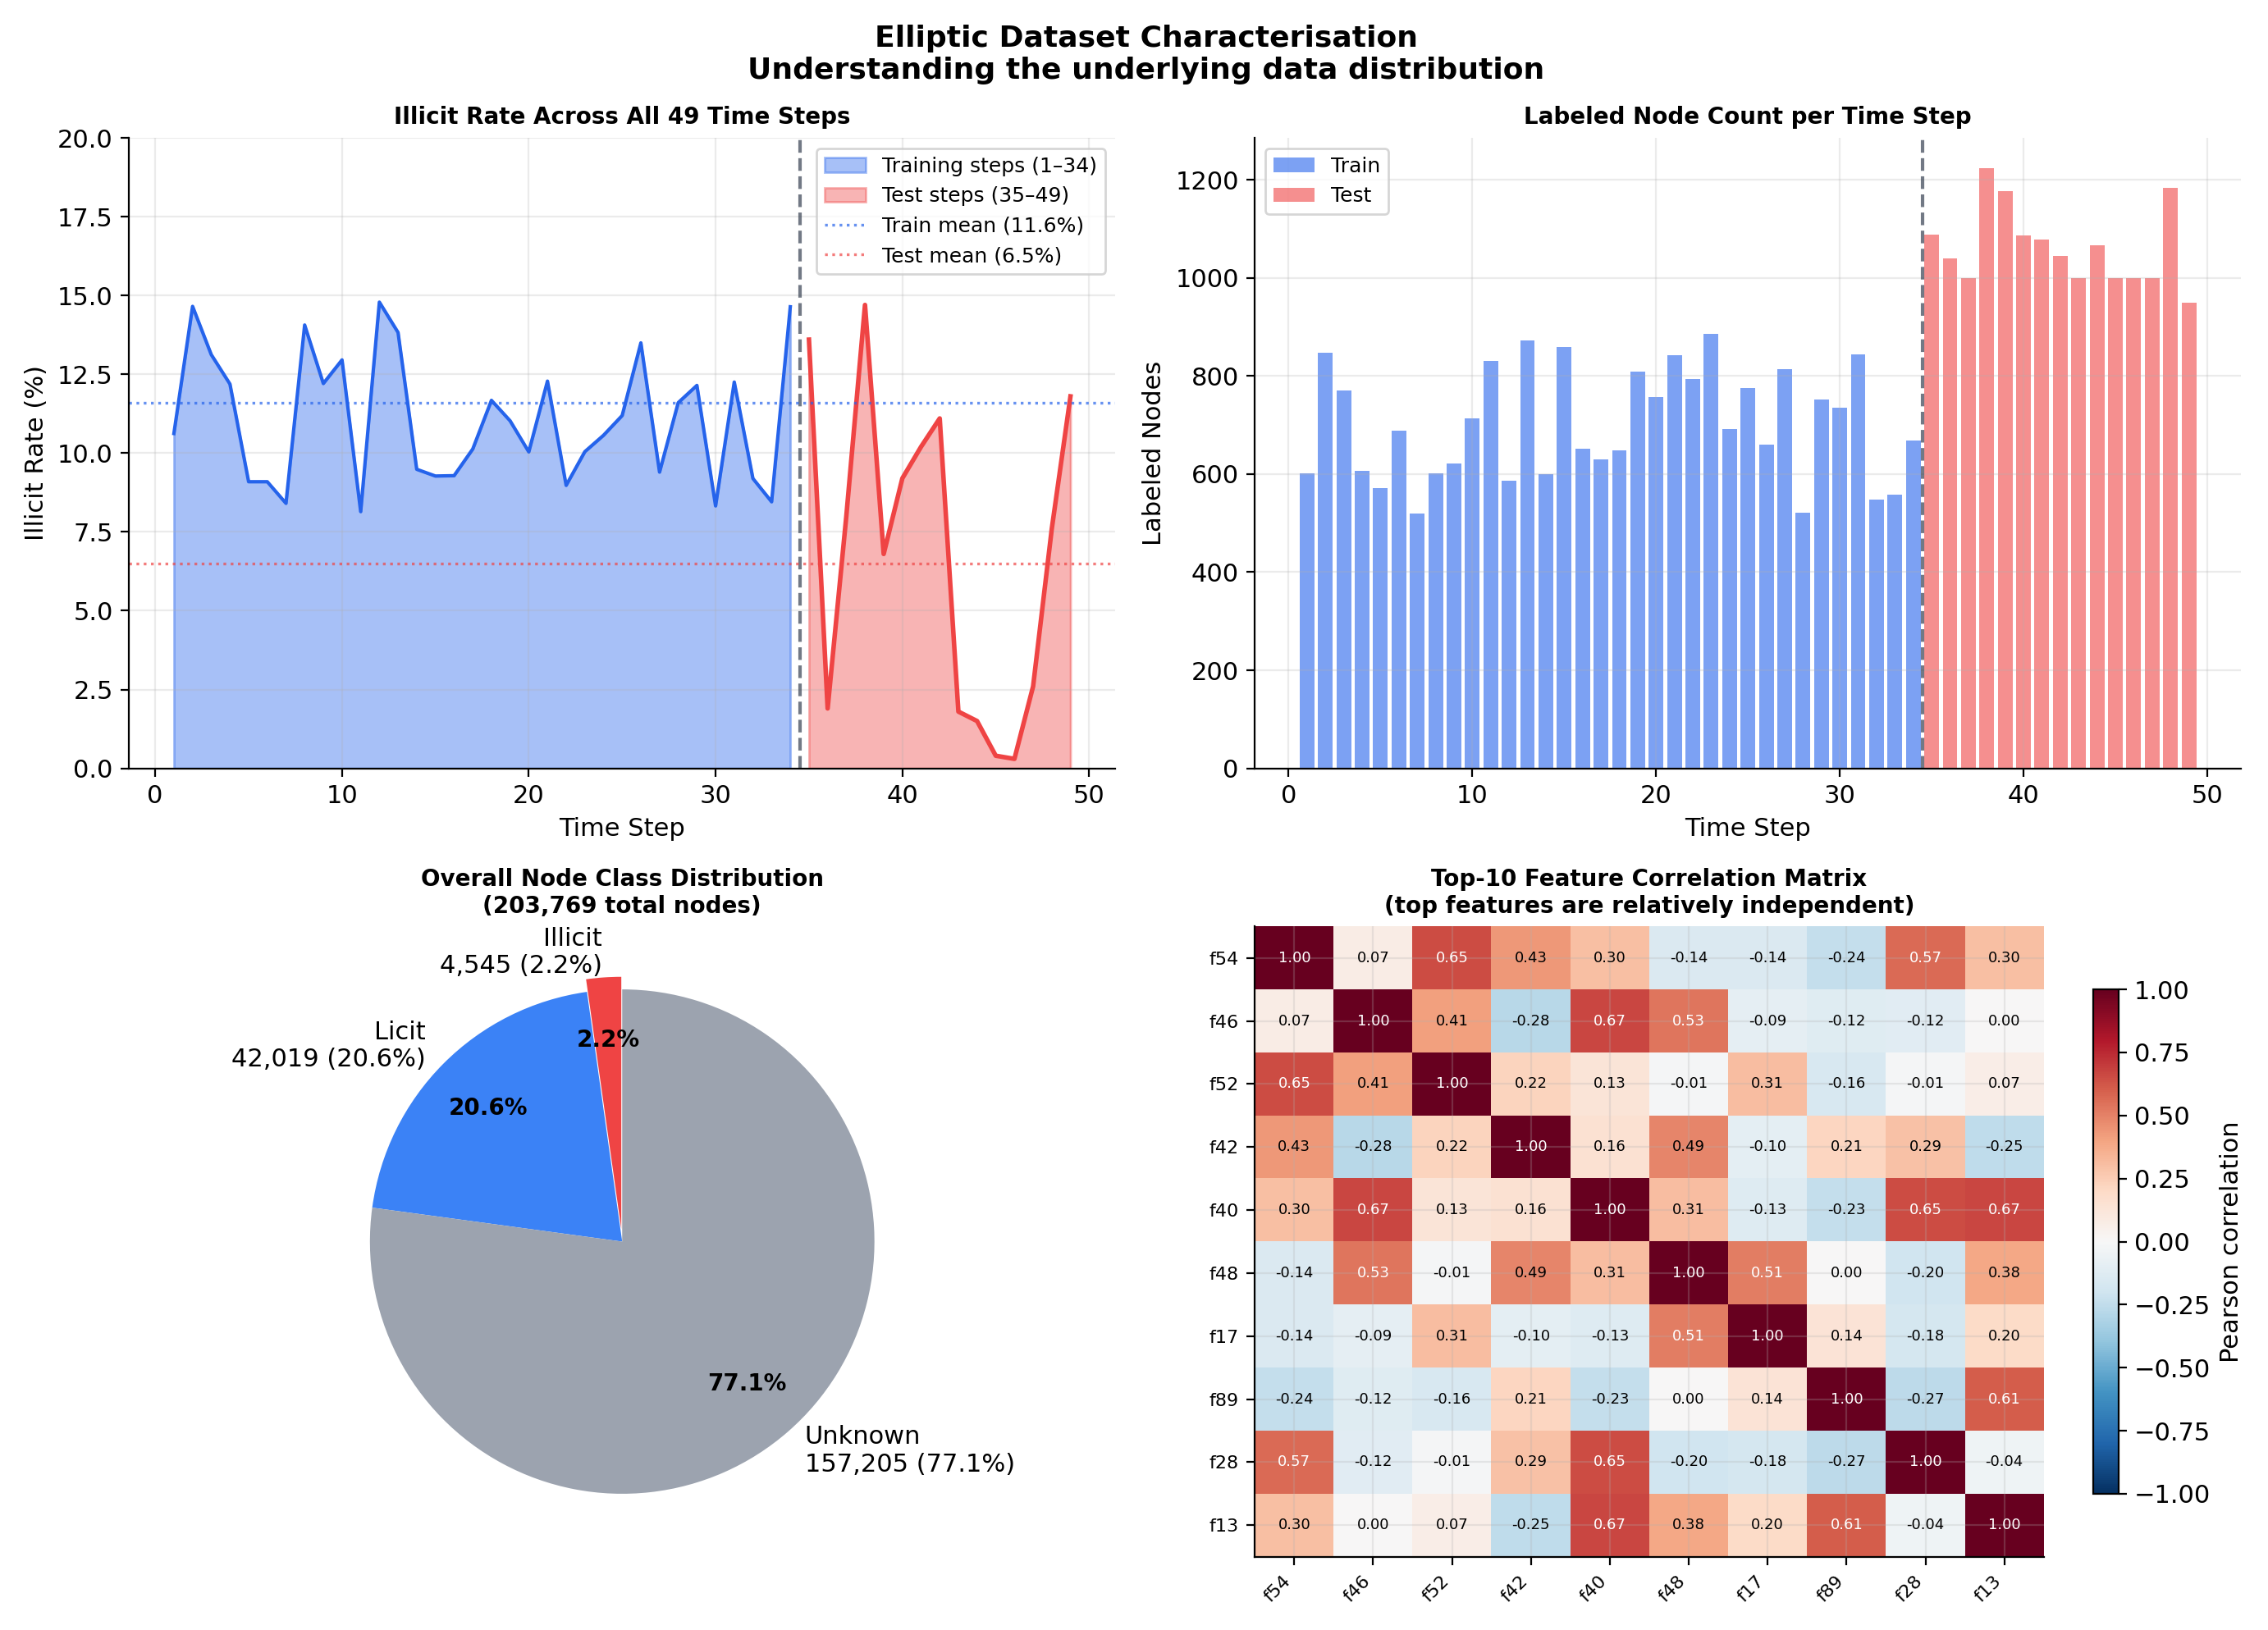
\includegraphics[width=\linewidth]{fig17_dataset_analysis.png}
\caption{Dataset characterisation. The train/test split coincides with
  a clear change in illicit-rate regime, and the most important features
  remain only moderately correlated rather than collapsing into a single
  redundant block.}
\label{fig:dataset_char}
\end{figure}

\subsection{Evaluation Protocol}

Primary metric: F1 on the illicit class (mean\,$\pm$\,std, 3 seeds).
Inductive evaluation via RandomNodeLoader (batch 512) prevents test-node
neighbourhood access during training. NeighborLoader is unavailable on
Apple M4 CPU without \texttt{torch-sparse}.

\section{Architectures and Training}
\label{sec:methods}

\textbf{MLP} (control): 3 hidden layers of size 128, BatchNorm, ReLU,
dropout 0.5. Ignores graph structure; 61,187 parameters.

\textbf{GCN \cite{kipf2017}}: 2-layer GCN with symmetric degree
normalisation. Hidden 128.

\textbf{GraphSAGE \cite{hamilton2017}}: 3-layer mean-aggregation SAGE.
Linear(165$\to$256) + [SAGEConv + BN + ReLU + Drop]$\times$3.
Total 438,787 parameters.

\textbf{GAT \cite{velickovic2018}}: 3-layer, 4 attention heads, edge
dropout 0.2, hidden 256. Total 243,715 parameters.

\textbf{EvolveGCN \cite{pareja2020evolvegcn}}: GRU-evolved GCN weights.
CPU-limited: 46,564-node subgraph, 8 sampled training snapshots.

Three imbalance strategies: Baseline CE (equal weights); Weighted CE
($w_c = \sqrt{N_\text{labeled}/2N_c}$, $w_\text{illicit}\approx 2.08$,
20-epoch linear warmup); Graph Augmentation (30 fraud 1-hop ego-graph
clones, $\sigma\!=\!0.02$, attached as isolated training components).

Training: AdamW ($\text{lr}=10^{-3}$, wd$=5{\times}10^{-4}$),
CosineAnnealingLR, gradient clipping (max norm 1.0), early stopping
patience 30. Apple M4 CPU.

\section{Results}
\label{sec:results}

\subsection{Main Benchmark}

Table~\ref{tab:main_results} presents all results; Fig.~\ref{fig:main_results}
visualises them as grouped bars. The MLP (F1\,=\,0.744) beats GraphSAGE
(F1\,=\,0.697) by 4.7\,pp outside both models' standard deviations.
GCN exhibits a precision paradox: precision 0.89--0.93 but recall
only 0.29--0.32, confirming it almost never predicts fraud. Strategy
matters little for SAGE (all within $\pm$std) but more for GAT (Weighted
CE lifts recall $\sim$5\,pp).

\begin{figure*}[!t]
\centering
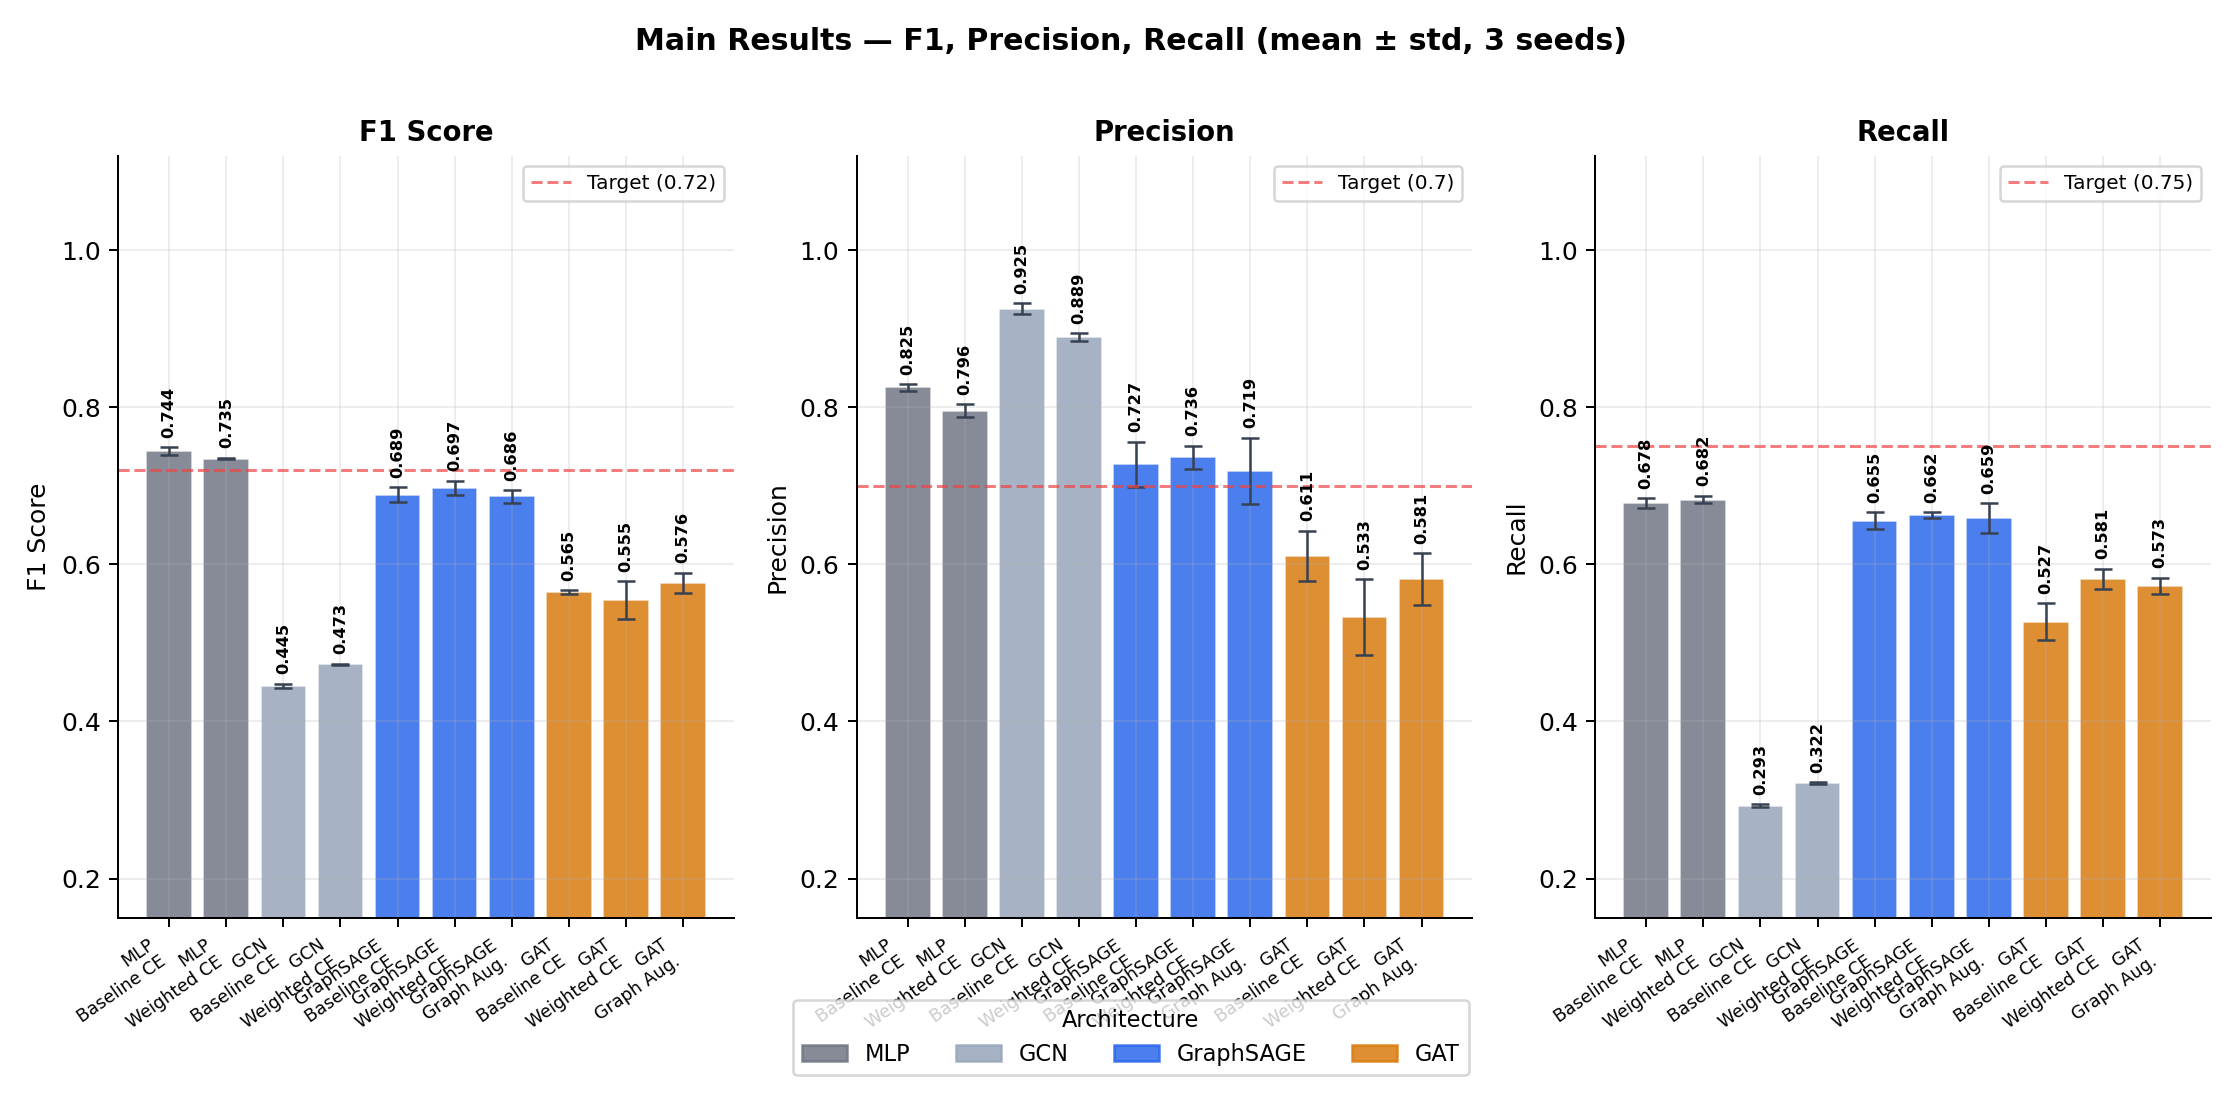
\includegraphics[width=0.96\textwidth]{fig1_main_results.png}
\caption{Main benchmark: F1, Precision, Recall (mean\,$\pm$\,std, 3 seeds).
  MLP achieves the highest F1. GCN's precision paradox is visible: very
  high precision but near-zero recall. GAT error bars are the widest due
  to attention instability under class imbalance. Red dashed lines mark
  target thresholds.}
\label{fig:main_results}
\end{figure*}

\begin{table*}[!t]
\centering
\caption{Benchmark Results (Mean $\pm$ Std, 3 Seeds). Bold: column best.
  No configuration reaches the 0.75 recall target due to temporal collapse.}
\label{tab:main_results}
\small
\setlength{\tabcolsep}{5pt}
\begin{tabular}{llrrrr}
\toprule
\textbf{Model} & \textbf{Strategy}
  & \textbf{F1} & \textbf{Prec.}
  & \textbf{Recall} & \textbf{AUC} \\
\midrule
\multirow{2}{*}{MLP}
  & Baseline CE
    & $\mathbf{0.744\pm0.005}$ & $\mathbf{0.825\pm0.004}$
    & $0.678\pm0.006$ & $0.891\pm0.001$ \\
  & Weighted CE
    & $0.735\pm0.001$ & $0.796\pm0.008$
    & $0.682\pm0.005$ & $\mathbf{0.893\pm0.006}$ \\
\midrule
\multirow{2}{*}{GCN}
  & Baseline CE
    & $0.445\pm0.003$ & $0.925\pm0.007$
    & $0.293\pm0.002$ & $0.868\pm0.009$ \\
  & Weighted CE
    & $0.473\pm0.001$ & $0.889\pm0.005$
    & $0.322\pm0.001$ & $0.872\pm0.004$ \\
\midrule
\multirow{3}{*}{GraphSAGE}
  & Baseline CE
    & $0.689\pm0.009$ & $0.727\pm0.029$
    & $0.655\pm0.011$ & $0.867\pm0.006$ \\
  & Weighted CE
    & $0.697\pm0.009$ & $0.736\pm0.015$
    & $0.662\pm0.004$ & $0.868\pm0.003$ \\
  & Graph Aug.
    & $0.686\pm0.008$ & $0.719\pm0.042$
    & $0.659\pm0.019$ & $0.861\pm0.007$ \\
\midrule
\multirow{3}{*}{GAT}
  & Baseline CE
    & $0.565\pm0.002$ & $0.611\pm0.032$
    & $0.527\pm0.023$ & $0.863\pm0.007$ \\
  & Weighted CE
    & $0.555\pm0.024$ & $0.533\pm0.048$
    & $\mathbf{0.581\pm0.013}$ & $0.855\pm0.004$ \\
  & Graph Aug.
    & $0.576\pm0.013$ & $0.581\pm0.033$
    & $0.573\pm0.010$ & $0.842\pm0.002$ \\
\bottomrule
\end{tabular}
\end{table*}

\subsection{Strategy Sensitivity and Seed Robustness}

The model ranking is more stable than the strategy ranking.
Fig.~\ref{fig:strategy_variance} combines the strategy view and the
seed-variance view. Weighted CE is the most consistently useful
intervention, while graph augmentation mainly changes the
precision-recall trade-off. MLP and GraphSAGE remain relatively stable
across seeds, whereas GAT shows noticeably wider variance.

\begin{figure*}[!t]
\centering
\begin{minipage}[b]{0.48\textwidth}
  \centering
  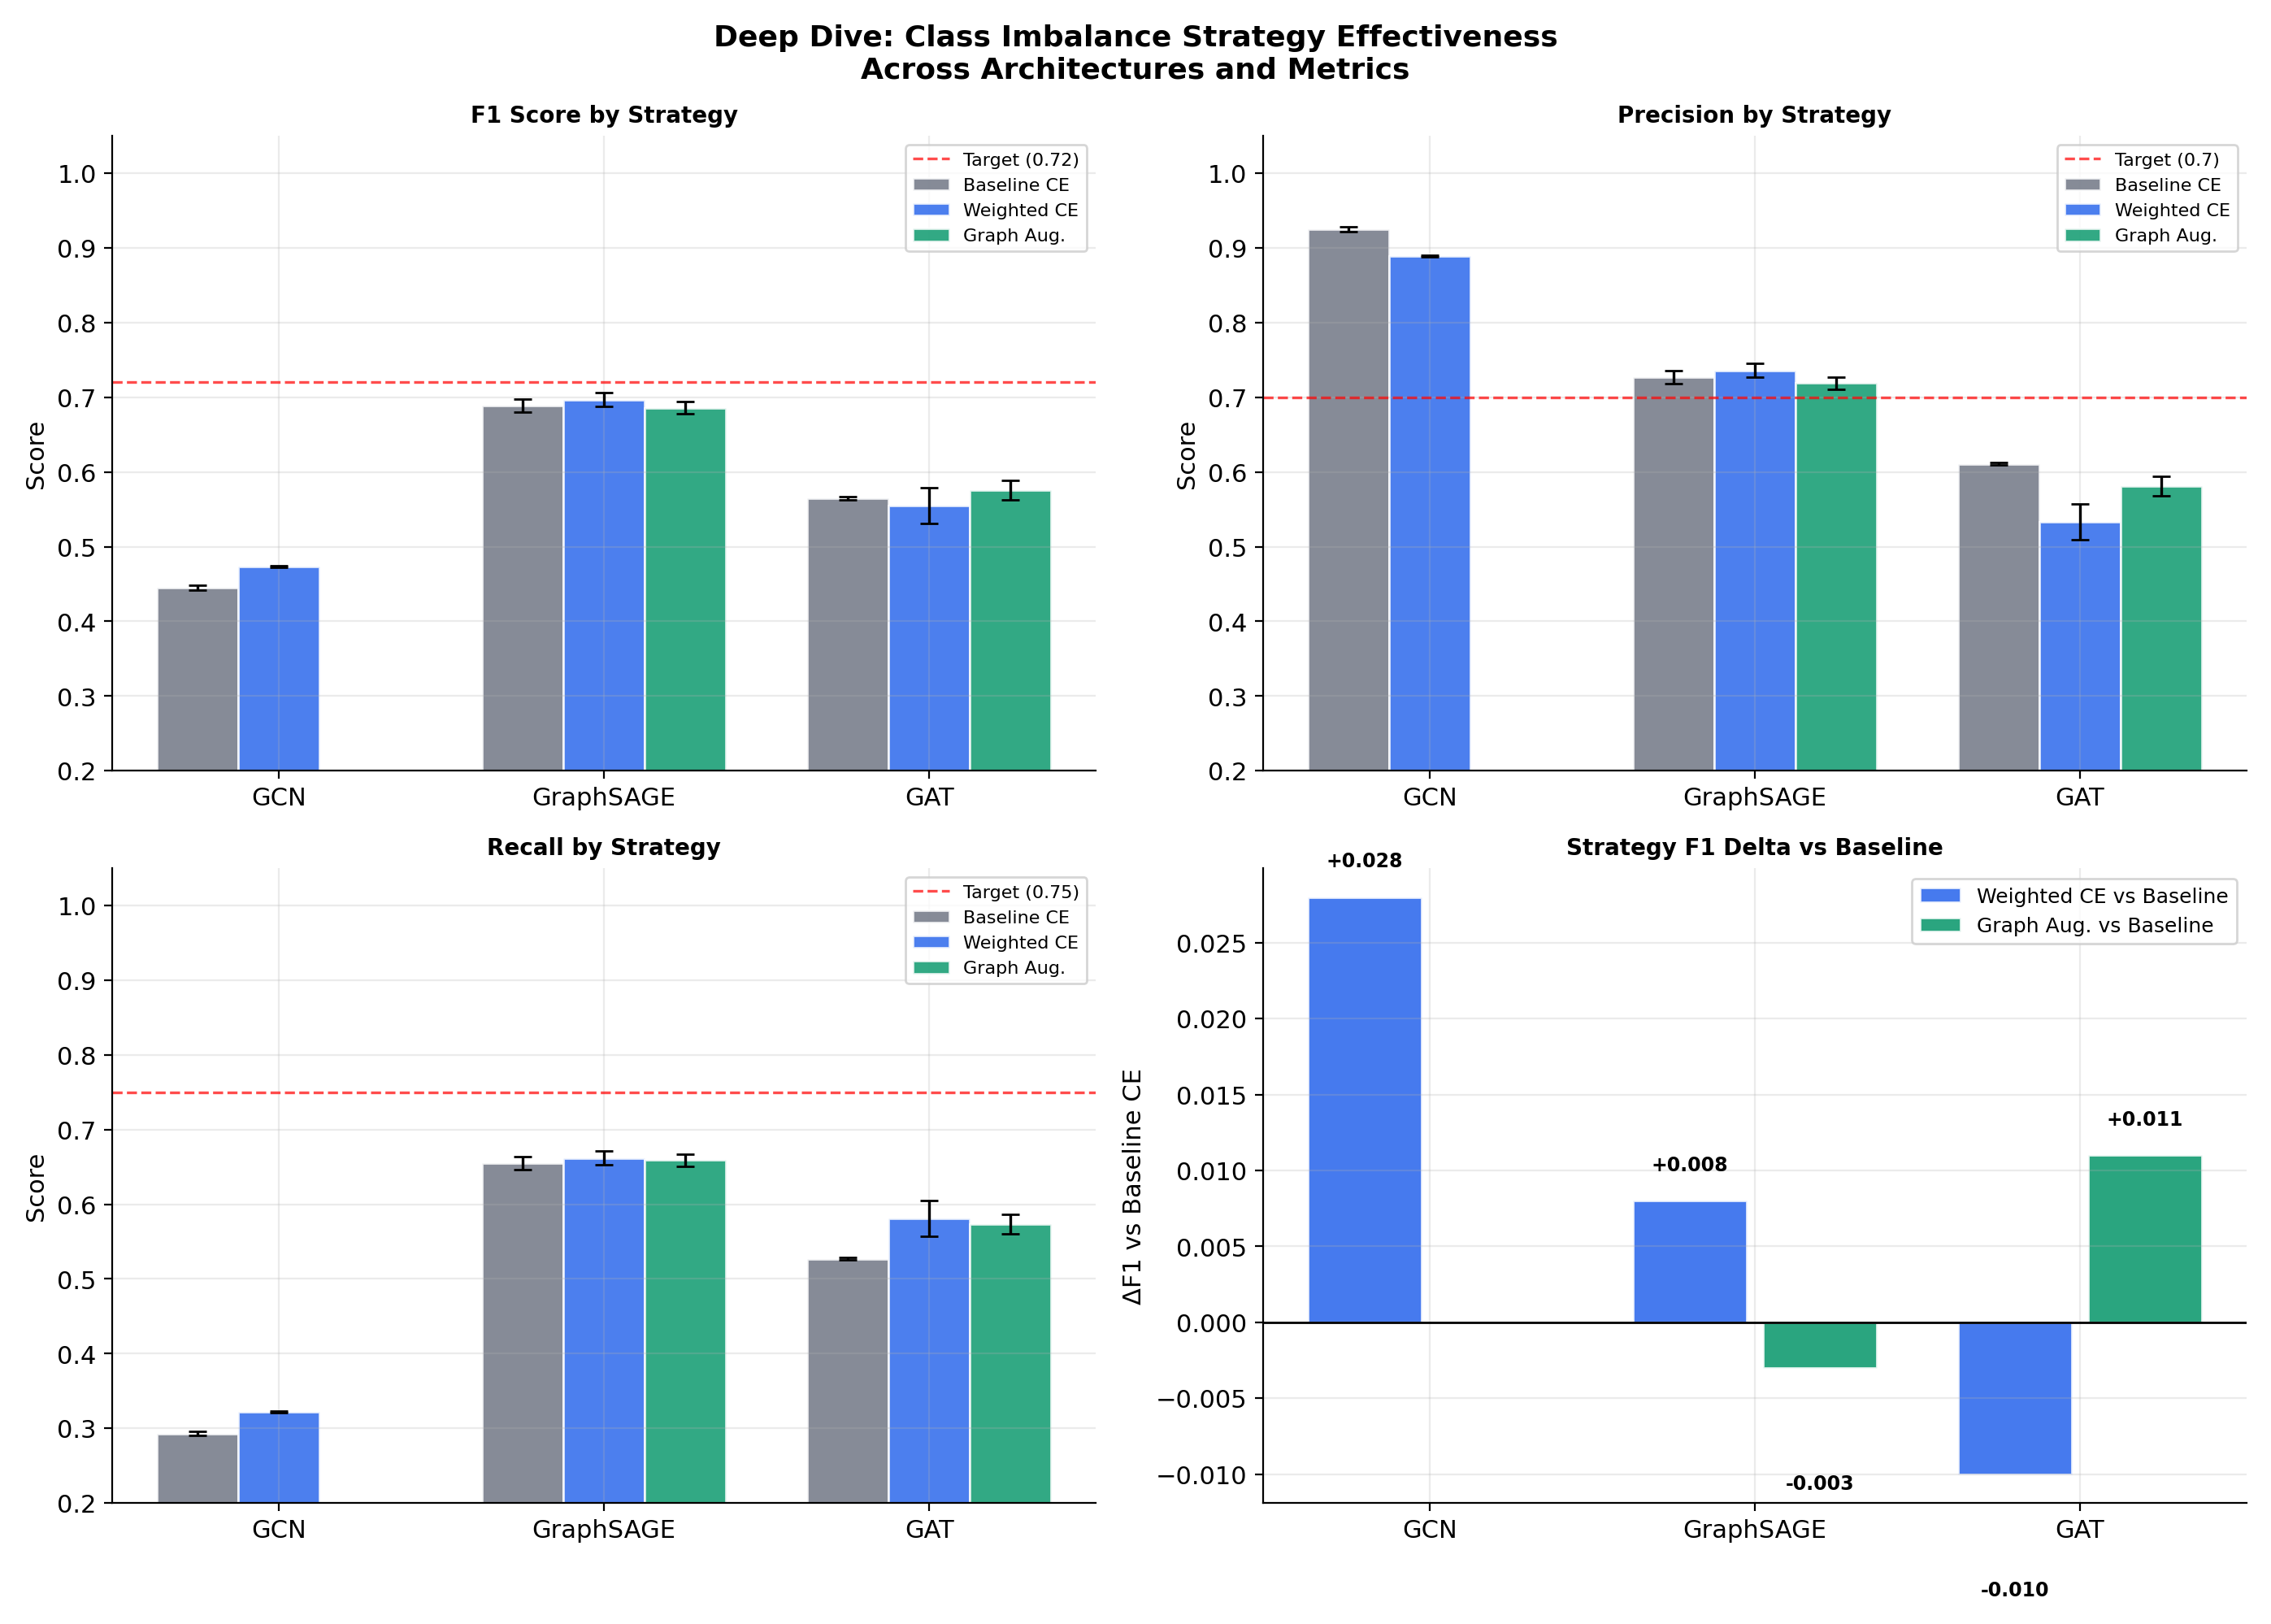
\includegraphics[width=\linewidth]{fig14_strategy_deep_dive.png}\\[-0.2em]
  \footnotesize\textbf{(a)} Strategy sensitivity across architectures.
\end{minipage}
\hfill
\begin{minipage}[b]{0.48\textwidth}
  \centering
  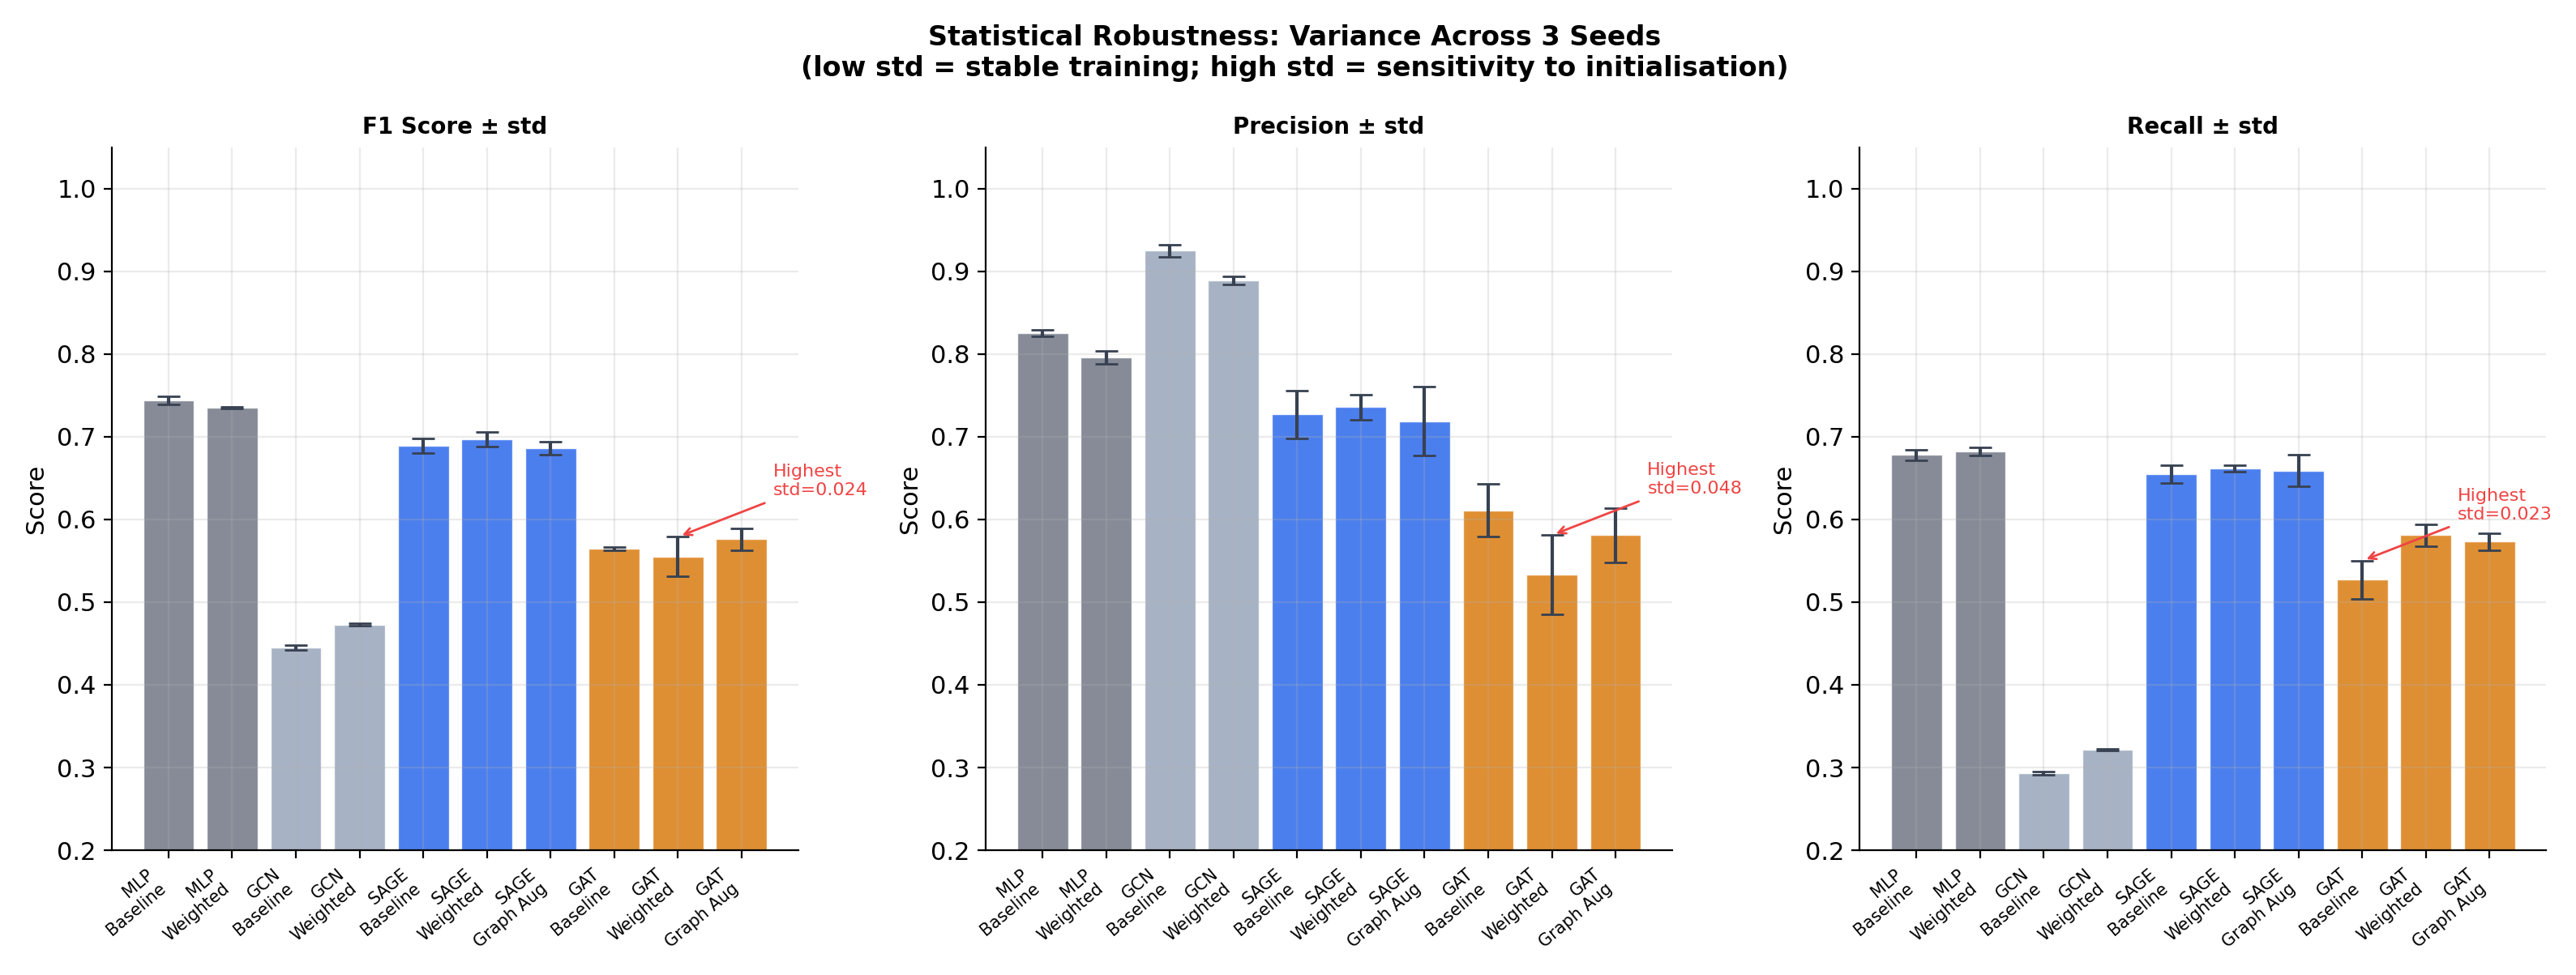
\includegraphics[width=\linewidth]{fig15_variance_analysis.png}\\[-0.2em]
  \footnotesize\textbf{(b)} Variance across the three training seeds.
\end{minipage}
\caption{Reorganising the benchmark by strategy and by seed confirms the
  same conclusion: architecture dominates the ranking, while GAT is the
  least stable family under imbalance.}
\label{fig:strategy_variance}
\end{figure*}

\subsection{Temporal Collapse}

Fig.~\ref{fig:temporal} shows per-step F1 versus true illicit rate.
Every configuration collapses identically after step~42. For GraphSAGE +
Weighted CE: mean F1 falls from 0.799 (steps 35--42) to 0.012 (steps
43--49). This is a recall failure: predicted fraud rate drops from 8.2\,\%
to 1.7\,\%, confirming models stop predicting fraud rather than becoming
confused.

\begin{figure*}[!t]
\centering
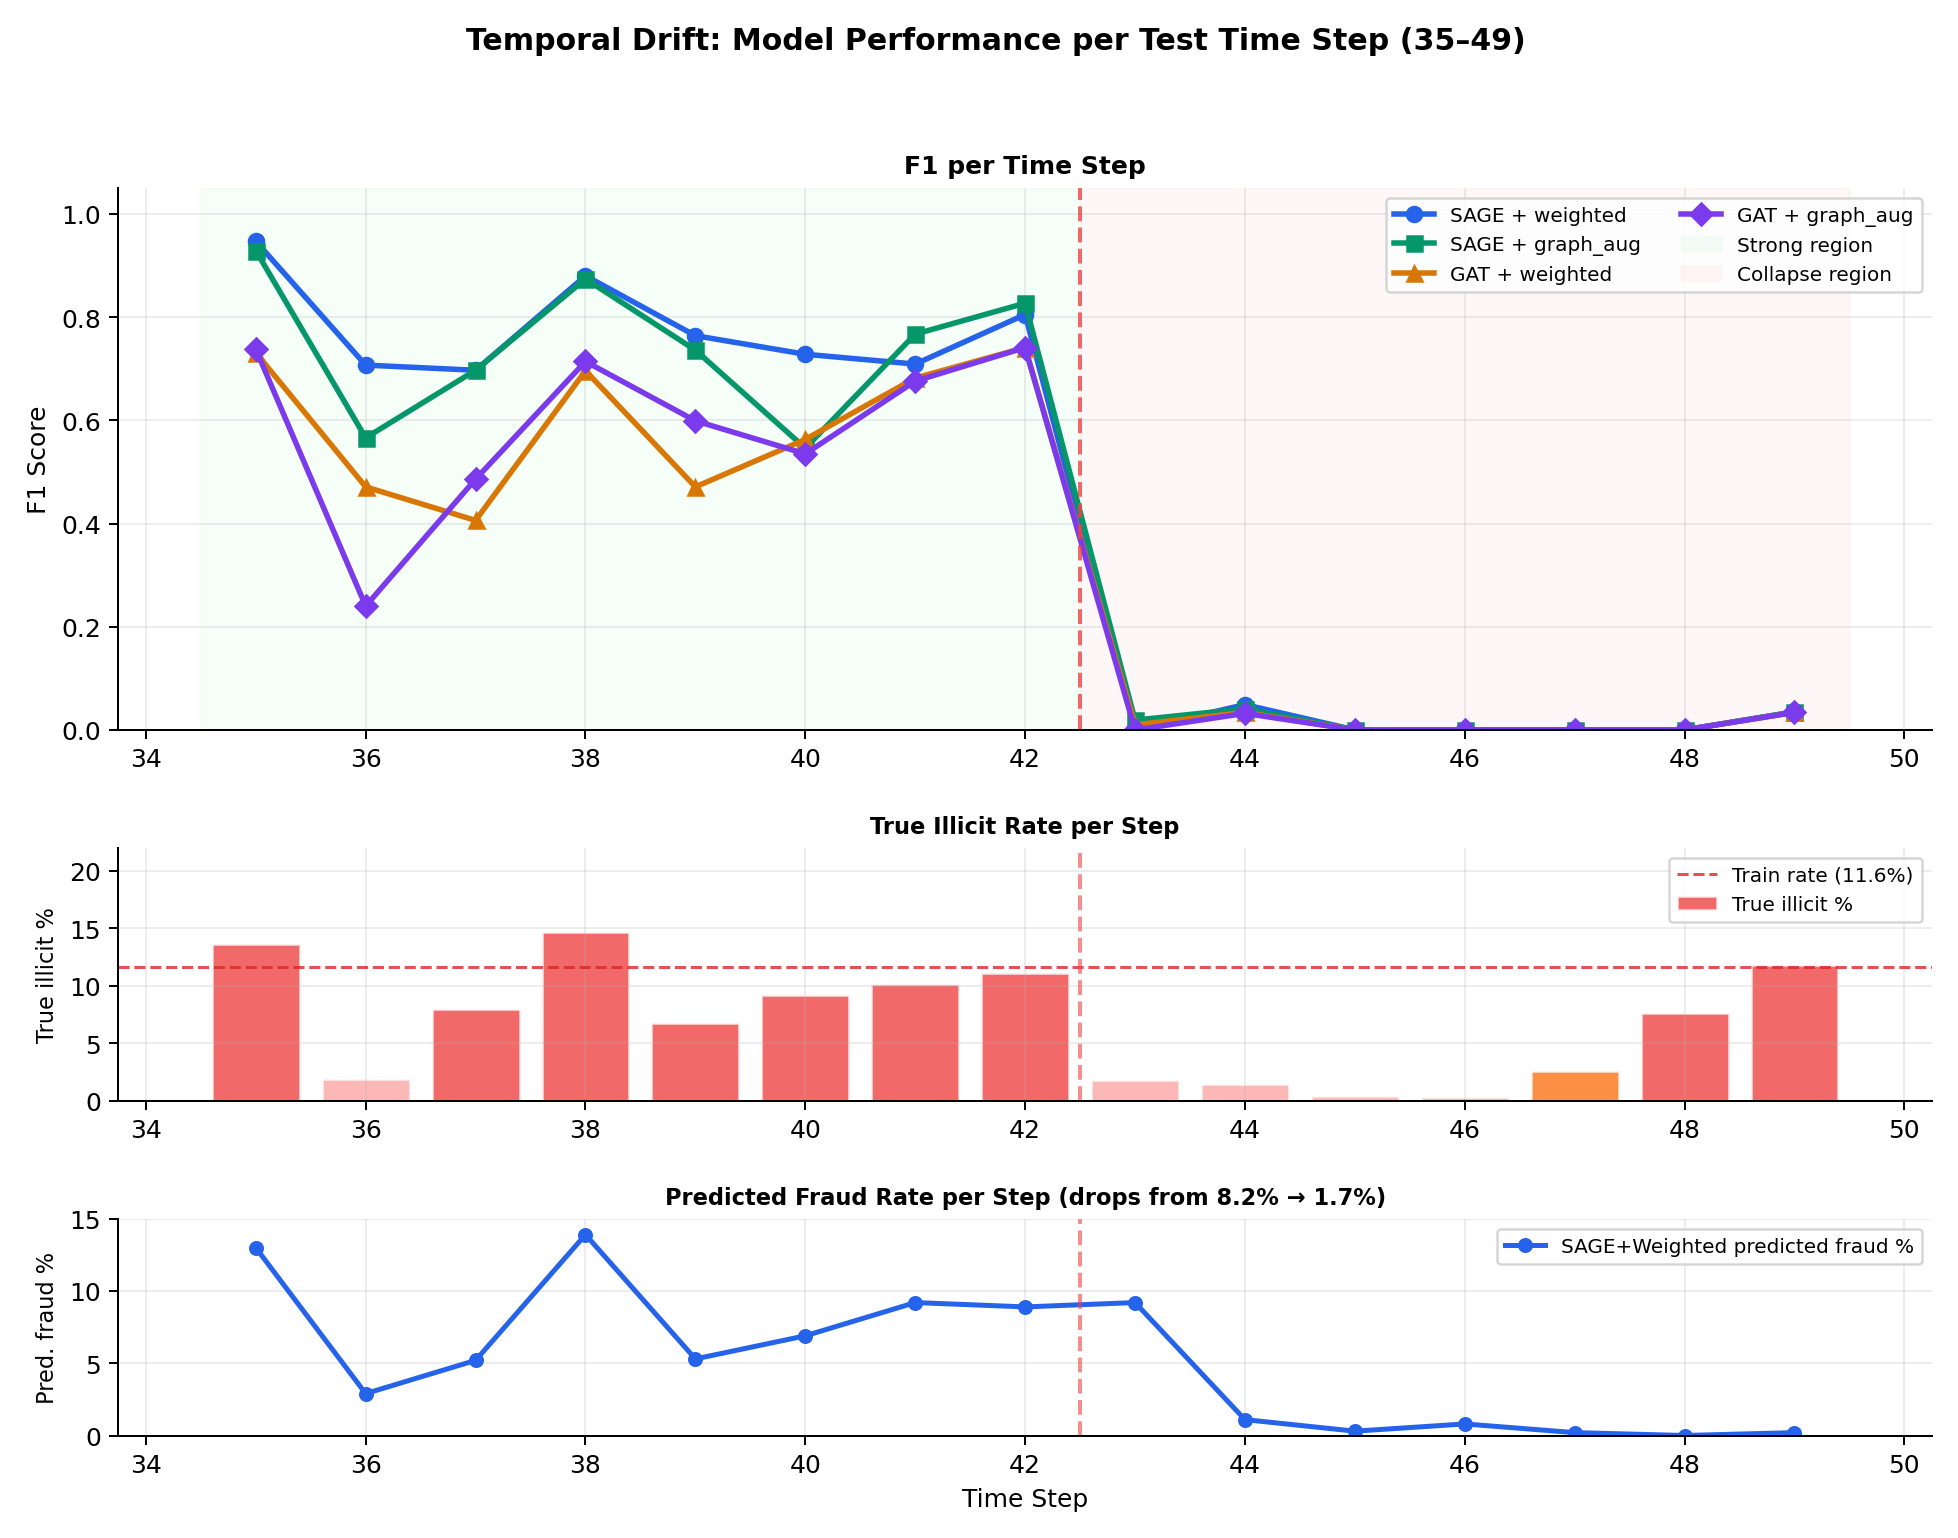
\includegraphics[width=0.96\textwidth]{fig2_temporal_drift.png}
\caption{Per-step F1 (top) versus true illicit rate (bottom). All
  configurations collapse identically after step~42, directly corresponding
  to the fraud-rate drop. The collapse is driven by distributional shift,
  not by architectural differences.}
\label{fig:temporal}
\end{figure*}

Table~\ref{tab:temporal_detail} gives full per-step numbers for
GraphSAGE + Weighted CE. Step~46 has only 3 fraud nodes among 960
labeled transactions (0.3\,\%)---the model correctly stops predicting
fraud at that base rate, but this renders it useless.

\begin{table}[!t]
\centering
\caption{Per-Step Metrics for GraphSAGE + Weighted CE}
\label{tab:temporal_detail}
\scriptsize
\setlength{\tabcolsep}{4pt}
\begin{tabular}{crrrrr}
\toprule
\textbf{Step} & \textbf{True\,\%} & \textbf{F1}
  & \textbf{Prec.} & \textbf{Recall} & \textbf{Pred\,\%} \\
\midrule
35 & 13.6 & 0.947 & 0.966 & 0.929 & 13.0 \\
36 &  1.9 & 0.707 & 0.592 & 0.879 &  2.9 \\
37 &  8.0 & 0.697 & 0.885 & 0.575 &  5.2 \\
38 & 14.7 & 0.880 & 0.905 & 0.856 & 13.9 \\
39 &  6.8 & 0.764 & 0.873 & 0.679 &  5.3 \\
40 &  9.2 & 0.728 & 0.855 & 0.634 &  6.9 \\
41 & 10.2 & 0.709 & 0.750 & 0.672 &  9.2 \\
42 & 11.1 & 0.805 & 0.906 & 0.724 &  8.9 \\
\midrule
43 &  1.8 & 0.000 & 0.000 & 0.000 &  9.2 \\
44 &  1.5 & 0.049 & 0.059 & 0.042 &  1.1 \\
45 &  0.4 & 0.000 & 0.000 & 0.000 &  0.3 \\
46 &  0.3 & 0.000 & 0.000 & 0.000 &  0.8 \\
47 &  2.6 & 0.000 & 0.000 & 0.000 &  0.2 \\
48 &  7.6 & 0.000 & 0.000 & 0.000 &  0.0 \\
49 & 11.8 & 0.035 & 1.000 & 0.018 &  0.2 \\
\midrule
Mean 35--42 & & \textbf{0.799} & 0.841 & 0.743 & 8.2 \\
Mean 43--49 & & \textbf{0.012} & 0.151 & 0.009 & 1.7 \\
\bottomrule
\end{tabular}
\end{table}

\subsection{PR Curves and Confusion Matrices}

SAGE + Graph Aug.\ achieves the highest average precision (AP\,=\,0.607),
suggesting better fraud-probability ranking even at the same aggregate F1.
Confusion matrices show SAGE produces fewer false negatives
(FN\,=\,388) than GAT (FN\,=\,500--529). Full figures are in
Fig.~\ref{fig:pr_cm}.

\begin{figure*}[!t]
\centering
\begin{minipage}[b]{0.48\textwidth}
  \centering
  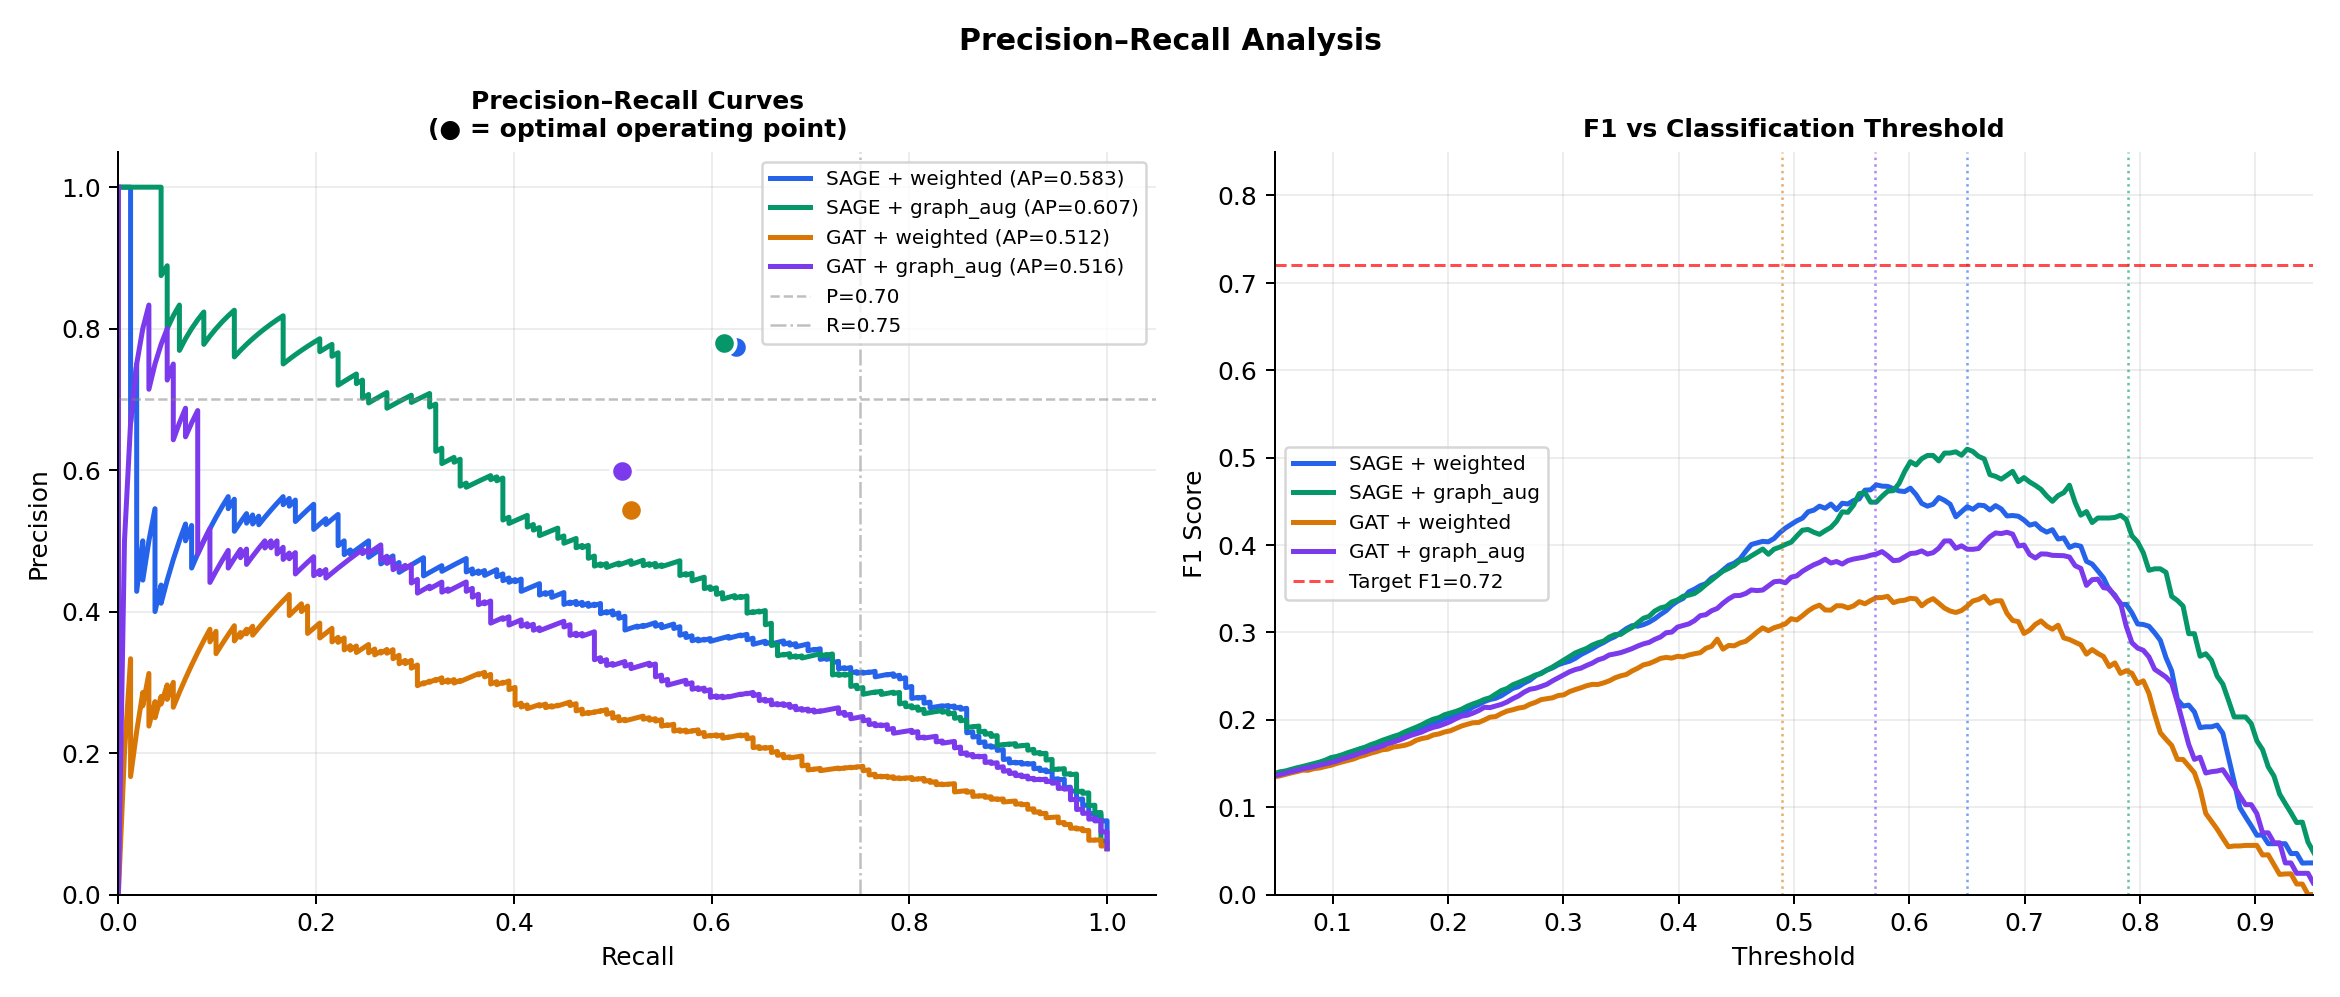
\includegraphics[width=\linewidth]{fig6_pr_curves.png}\\[-0.2em]
  \footnotesize\textbf{(a)} Precision-recall curves. No threshold simultaneously
  achieves precision $>$0.70 and recall $>$0.75.
\end{minipage}
\hfill
\begin{minipage}[b]{0.48\textwidth}
  \centering
  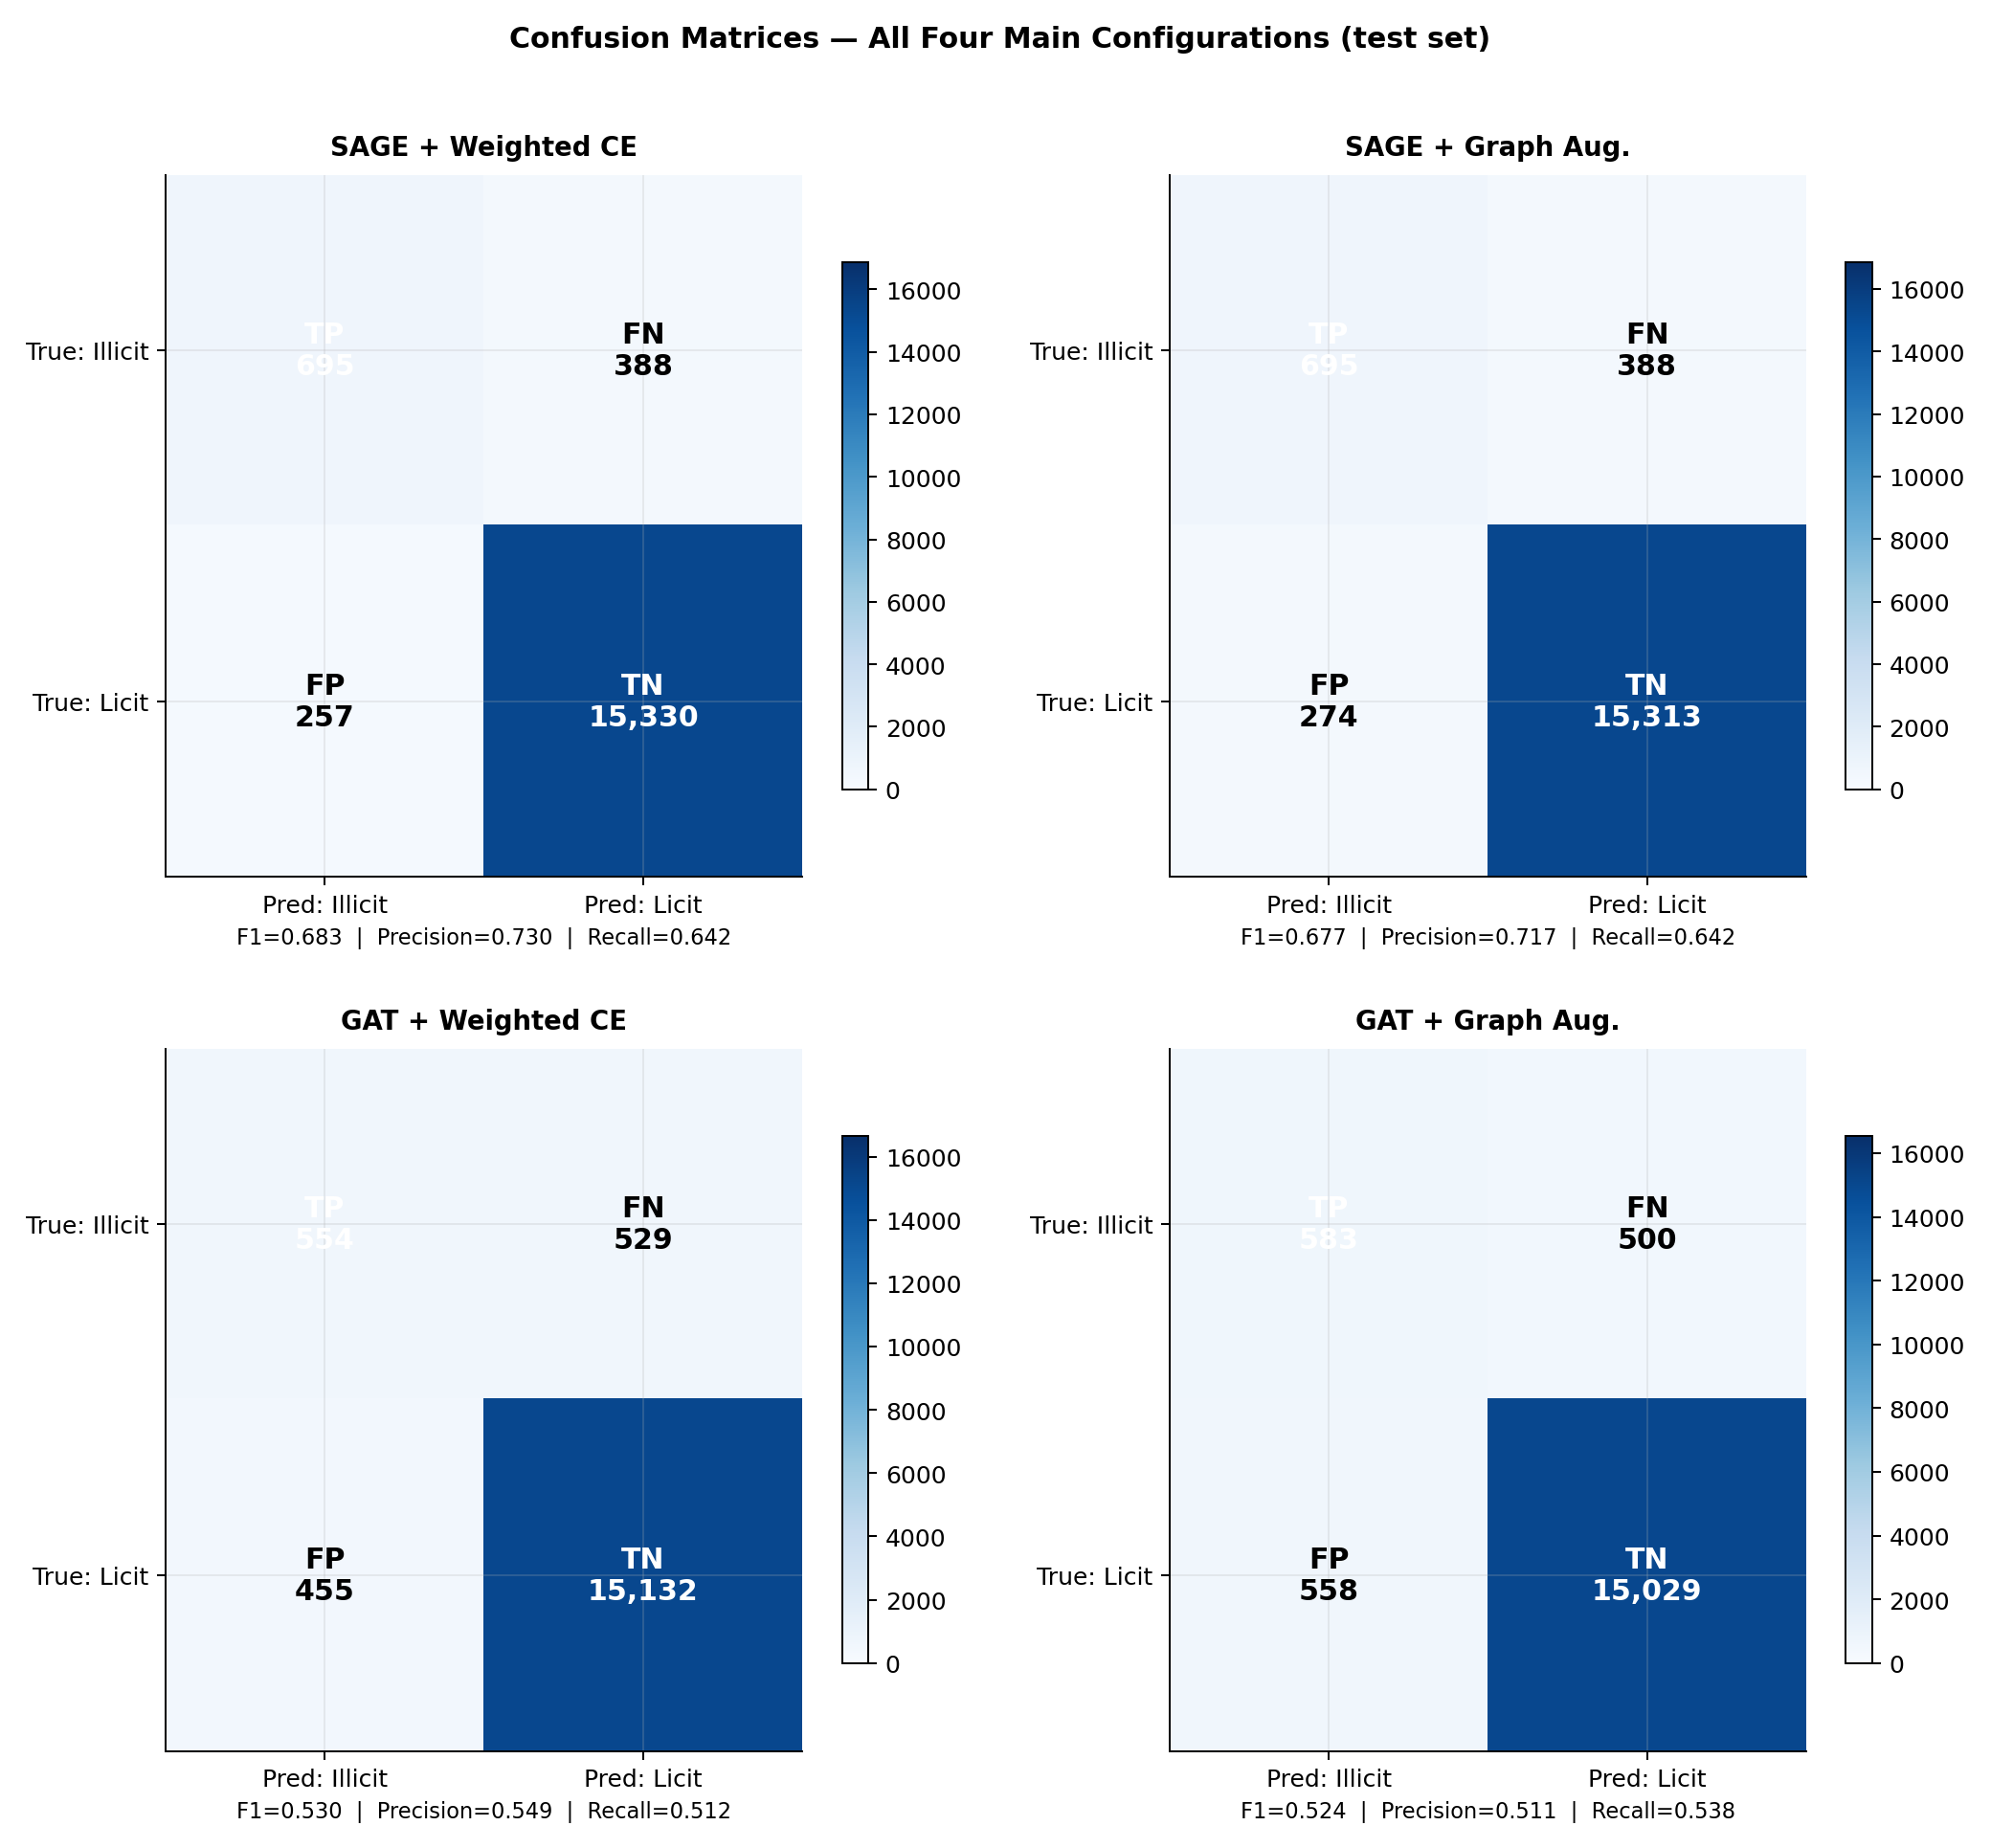
\includegraphics[width=\linewidth]{fig10_confusion_matrices.png}\\[-0.2em]
  \footnotesize\textbf{(b)} Confusion matrices. SAGE catches more fraud
  (fewer FN) than GAT but generates more false alarms.
\end{minipage}
\caption{Precision-recall (left) and confusion matrix analysis (right)
  for all four main configurations.}
\label{fig:pr_cm}
\end{figure*}

\subsection{Business Cost Analysis}

Under FN\,=\,\$50k and FP\,=\,\$2k, GAT + Graph Aug.\ achieves the lowest
total cost (\$18.5M) despite lower F1 than SAGE. It catches 83 more fraud
cases (583 vs.\ 500 TP) with only 103 additional false alarms (558 vs.\
455 FP). At a 25:1 cost asymmetry, each extra true positive outweighs
25 additional false alarms. Fig.~\ref{fig:biz} shows the full breakdown.

\begin{figure}[!t]
\centering
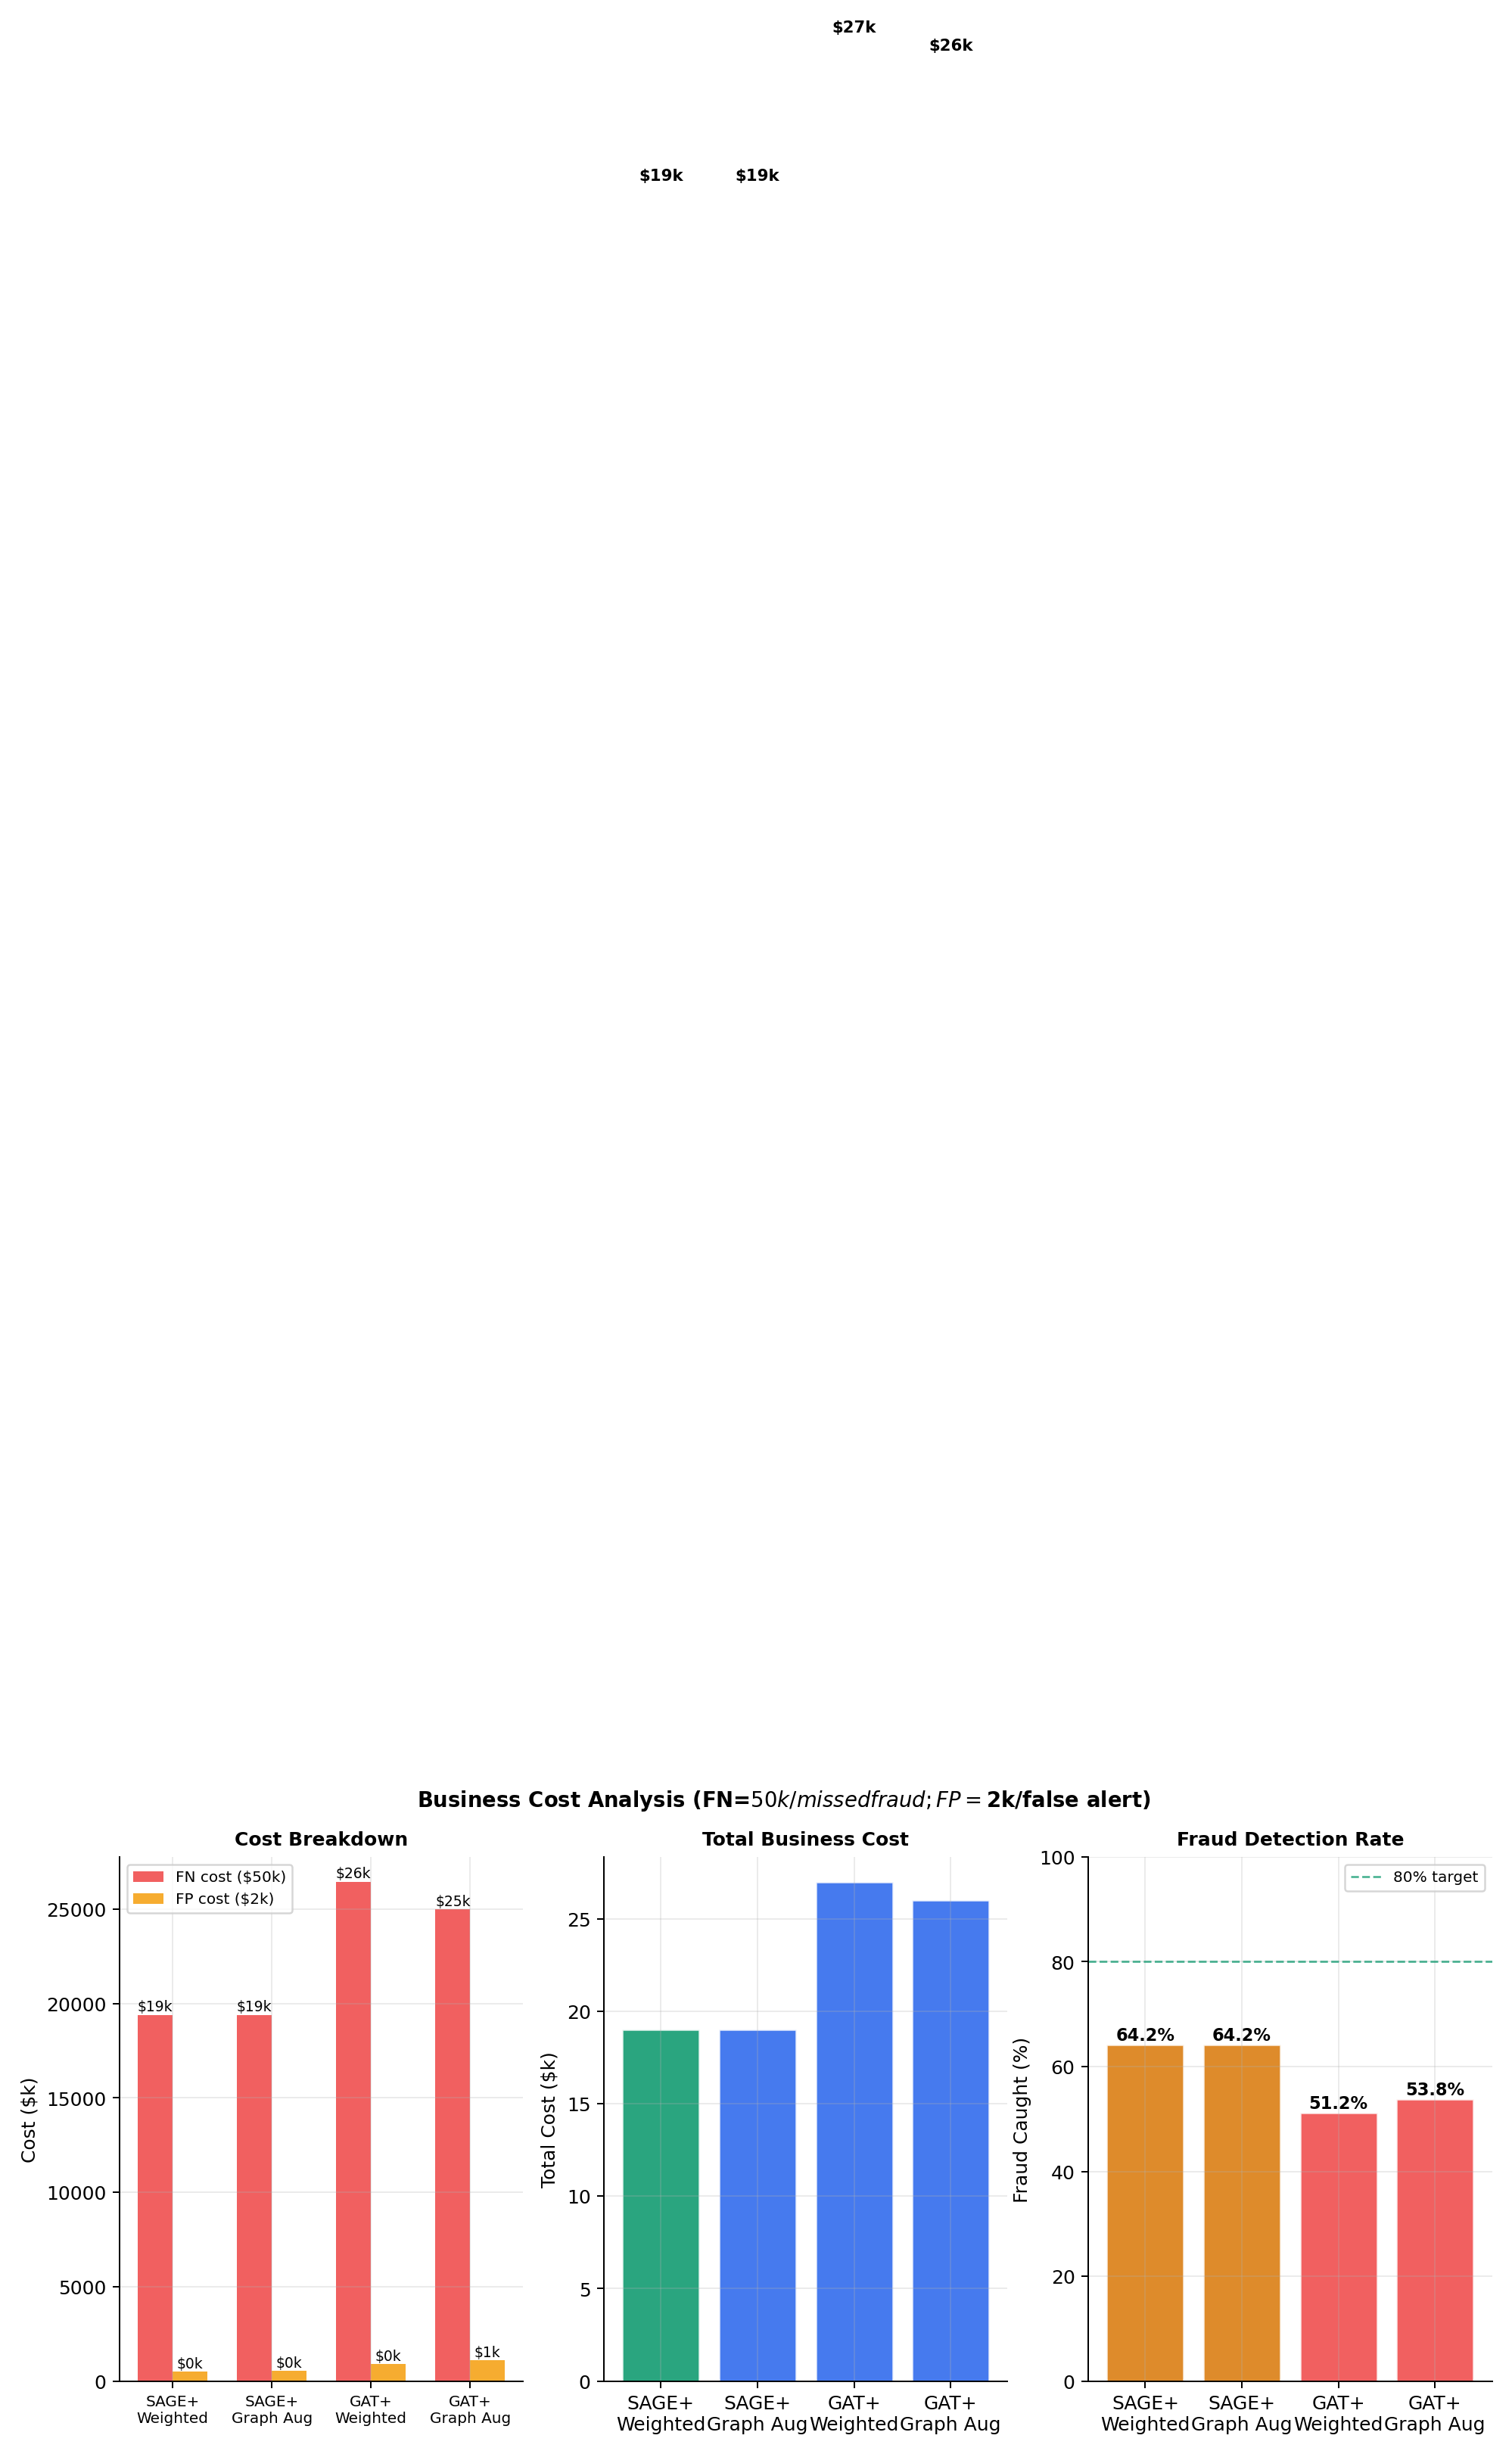
\includegraphics[width=0.90\linewidth]{fig7_business_cost.png}
\caption{Business cost analysis (FN\,=\,\$50k, FP\,=\,\$2k). GAT + Graph
  Aug.\ achieves the lowest operational cost despite lower aggregate F1,
  because catching more fraud outweighs the extra false-alarm cost.}
\label{fig:biz}
\end{figure}

\section{Analysis}
\label{sec:analysis}

\subsection{Feature Attribution and Graph-Advantage Ablation}

Random Forest importance on all 165 features (Fig.~\ref{fig:analysis_pair})
reveals that local features ($f_0$--$f_{93}$) account for 82.4\,\% of
total Gini importance. Aggregate neighbourhood features contribute only
17.6\,\% despite directly encoding 1-hop summaries. The top 17 features
explain 50\,\% of cumulative importance; the most important feature
(f54, importance 0.056) is local.

The implication is direct: the signal that matters for classification
is concentrated in features accessible to the MLP, while the GNNs'
structural component introduces topological patterns specific to the
training period that become misleading as fraud behaviour shifts.

The aggregate benchmark can obscure the fact that graph structure is not
uniformly harmful. Fig.~\ref{fig:ablation_advantage} shows the per-step
difference between GraphSAGE and the MLP baseline. The GNN is
competitive, and occasionally ahead, before the collapse boundary. Once
the test distribution moves into the low-fraud regime, the sign flips
and the MLP becomes the more reliable model.

\begin{figure*}[!t]
\centering
\begin{minipage}[b]{0.48\textwidth}
  \centering
  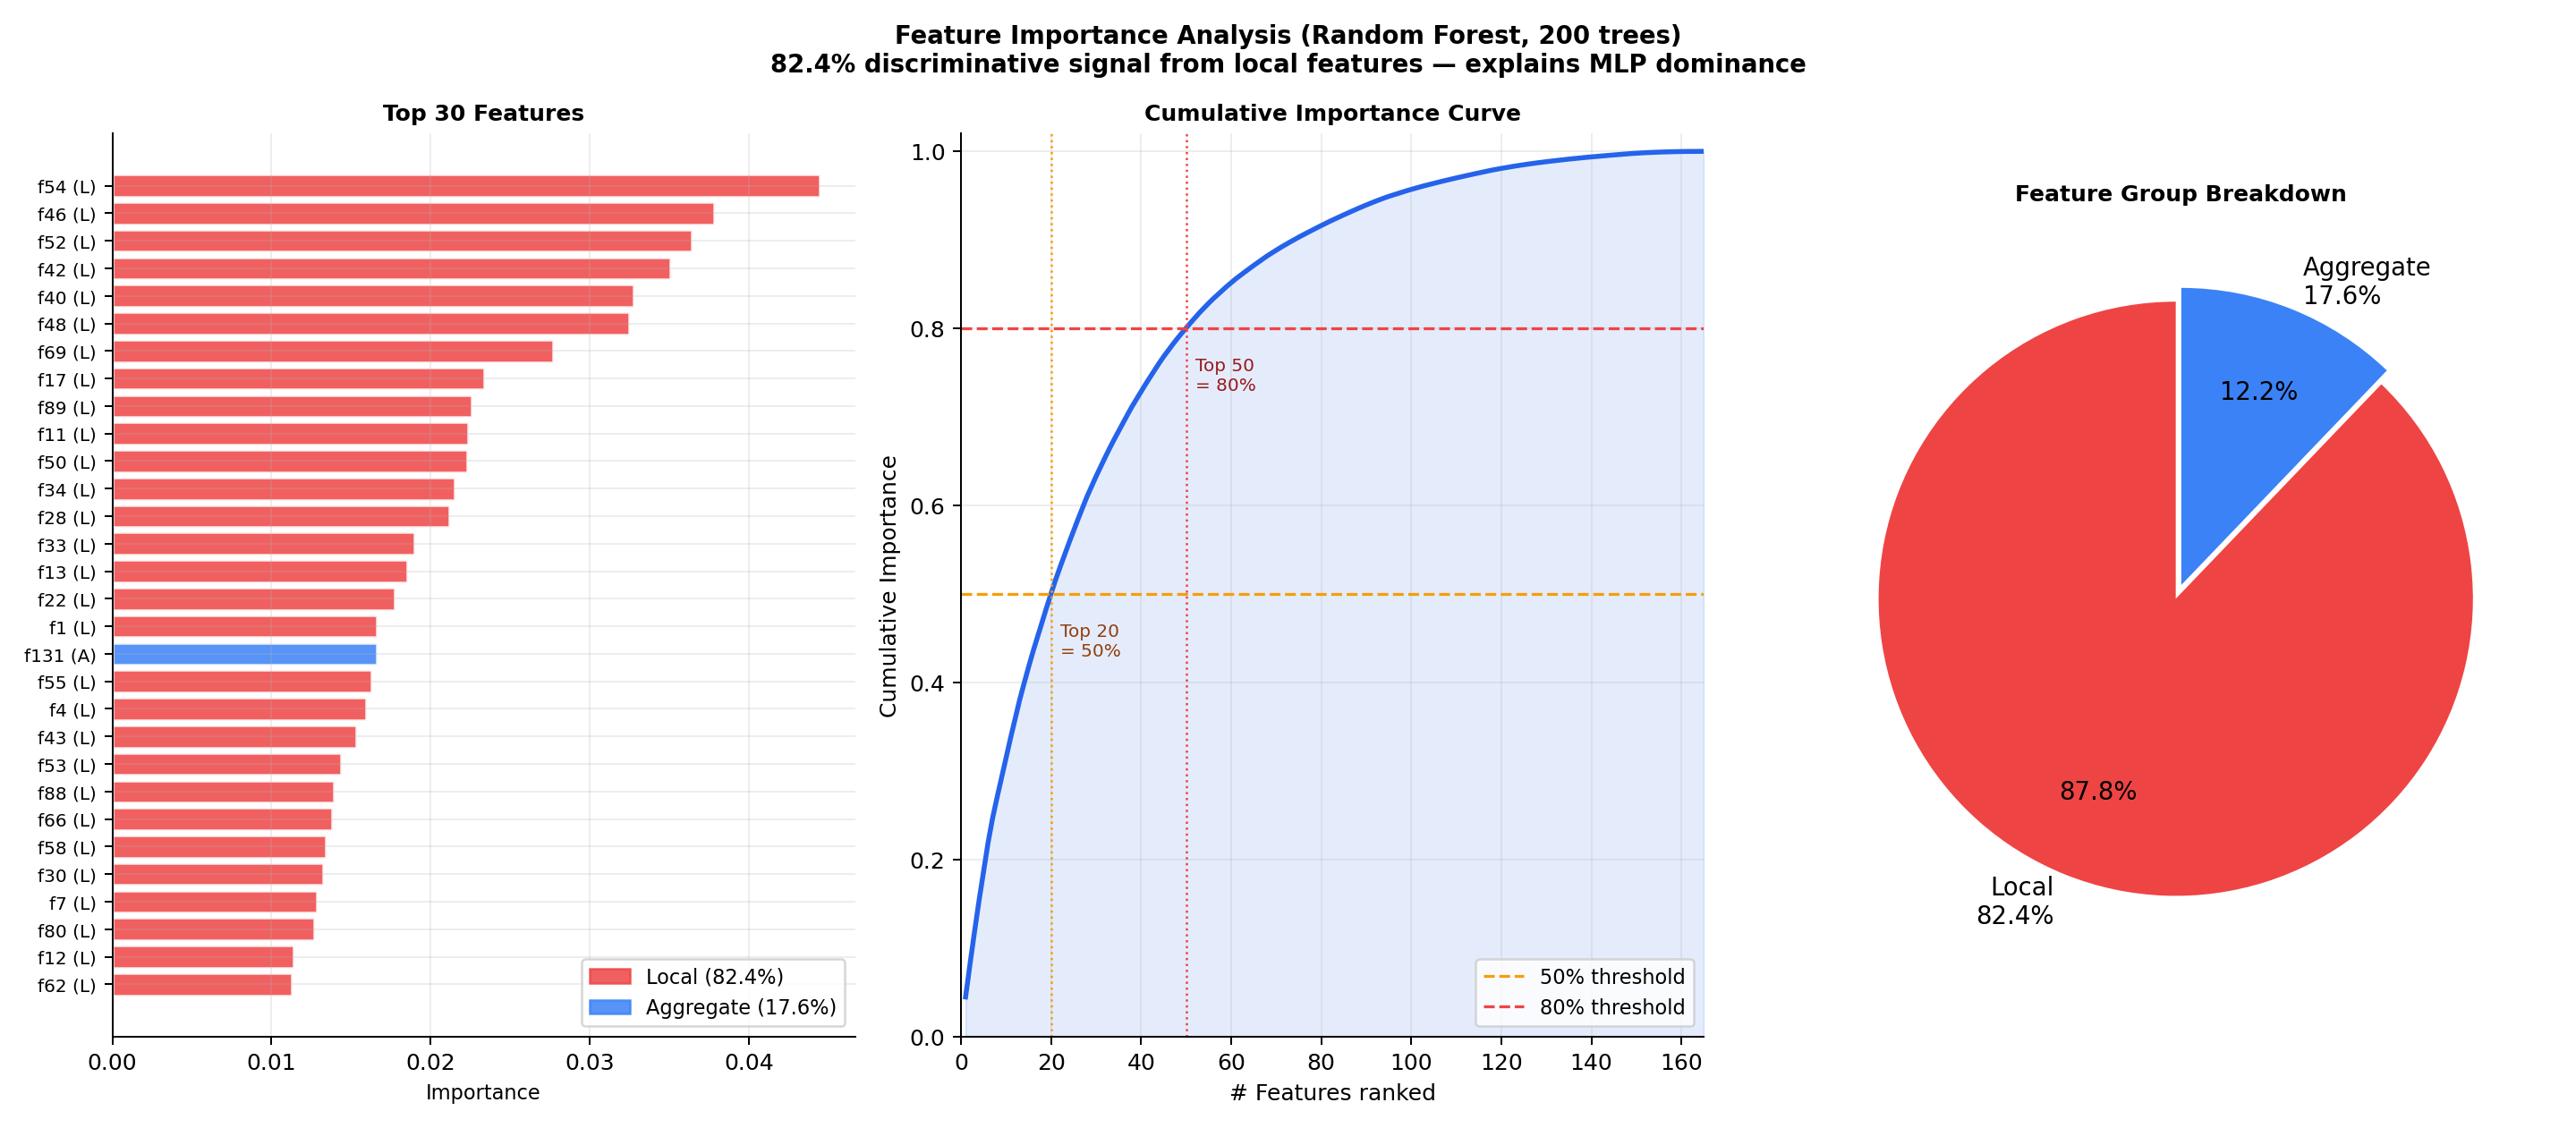
\includegraphics[width=\linewidth]{fig4_feature_importance.png}\\[-0.2em]
  \footnotesize\textbf{(a)} Feature importance. Local features dominate the stable signal.
\end{minipage}
\hfill
\begin{minipage}[b]{0.48\textwidth}
  \centering
  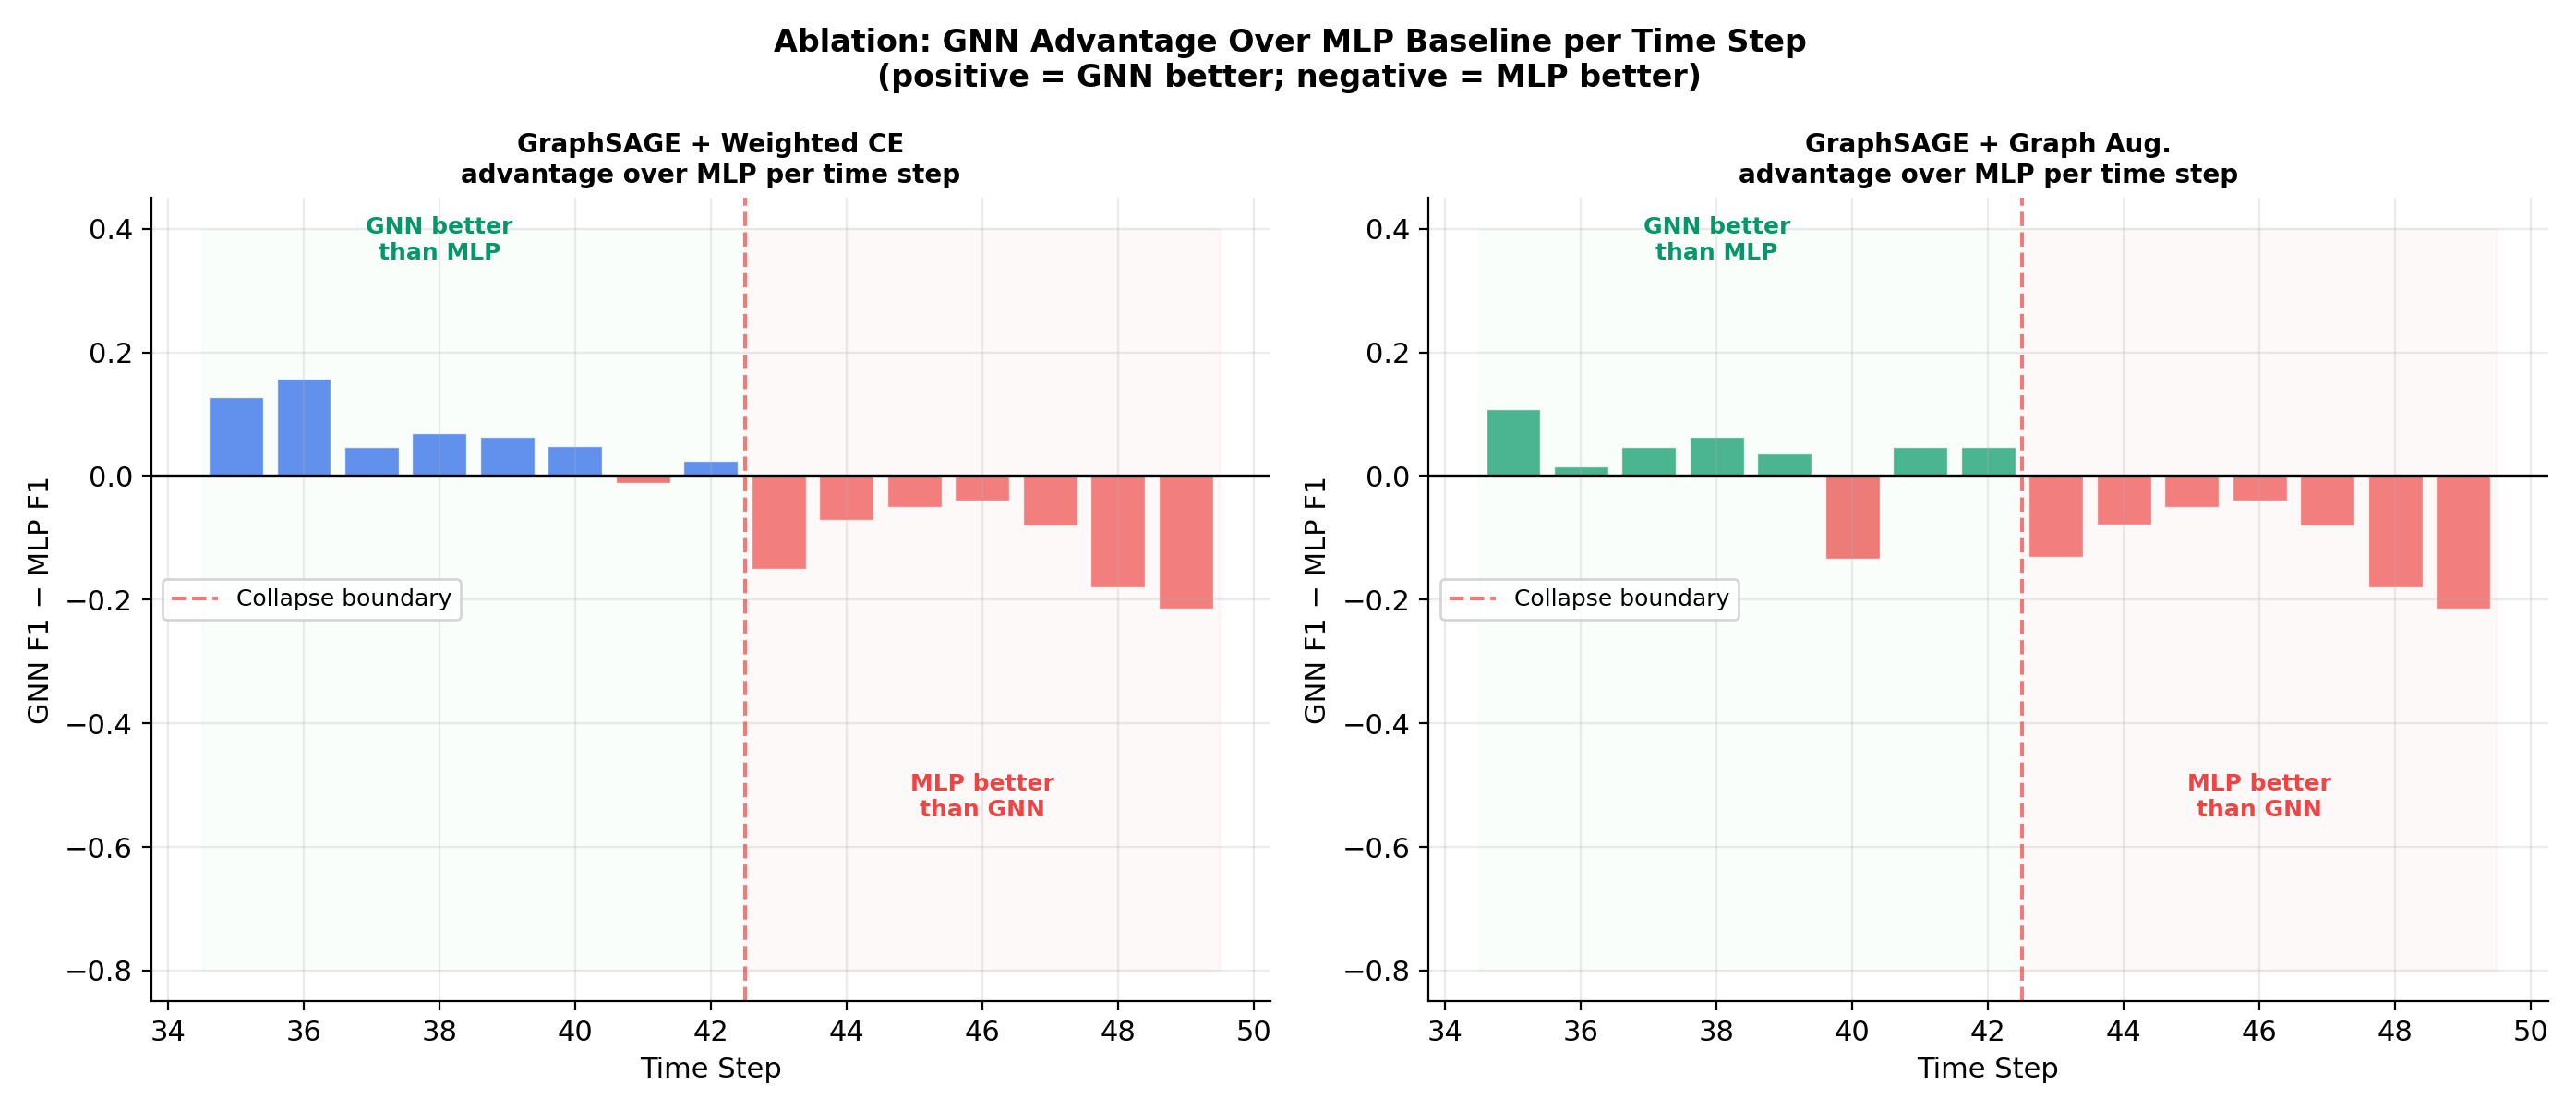
\includegraphics[width=\linewidth]{fig16_ablation_advantage.png}\\[-0.2em]
  \footnotesize\textbf{(b)} Per-step GraphSAGE advantage over the MLP baseline.
\end{minipage}
\caption{Analysis pair. Left: Random Forest importance shows that most
  discriminative power sits in local transaction features. Right: the
  graph-model advantage reverses after step~42, which is consistent with
  learned topology becoming stale under temporal shift.}
\label{fig:analysis_pair}
\label{fig:features}
\label{fig:ablation_advantage}
\end{figure*}

\subsection{Community Structure, Calibration, and Hardware}

Fraud community structure is genuine: fraud nodes have 54\,\% fraudulent
neighbours versus 0.56\,\% for licit nodes (96$\times$ ratio,
Fig.~\ref{fig:community}). GNNs do exploit this in steps 35--42. The
structure becomes a liability in steps 43--49 when learned topological
patterns from training no longer represent the test-period fraud distribution.

Fig.~\ref{fig:temp} shows $\Delta$F1\,=\,0 for all configurations after
temperature scaling ($T\in[1.07,1.27]$). Temperature scaling is
rank-preserving---it rescales probabilities but cannot move predictions
across the 0.5 threshold. The collapse is structural, not a calibration
artefact.

CPU-constrained EvolveGCN (F1\,=\,0.29) falls 0.48 points below the
published GPU result (F1\,=\,0.77). The gap isolates two constraints:
operating on the 46,564-node labeled subgraph rather than the full
203,769-node graph, and processing only 8 sampled training snapshots
rather than all 34. The training curve plateaus at epoch~30, consistent
with the GRU failing to learn smooth weight dynamics from sparse snapshots
(Fig.~\ref{fig:evolve}).

\begin{figure*}[!t]
\centering
\begin{minipage}[b]{0.32\textwidth}
  \centering
  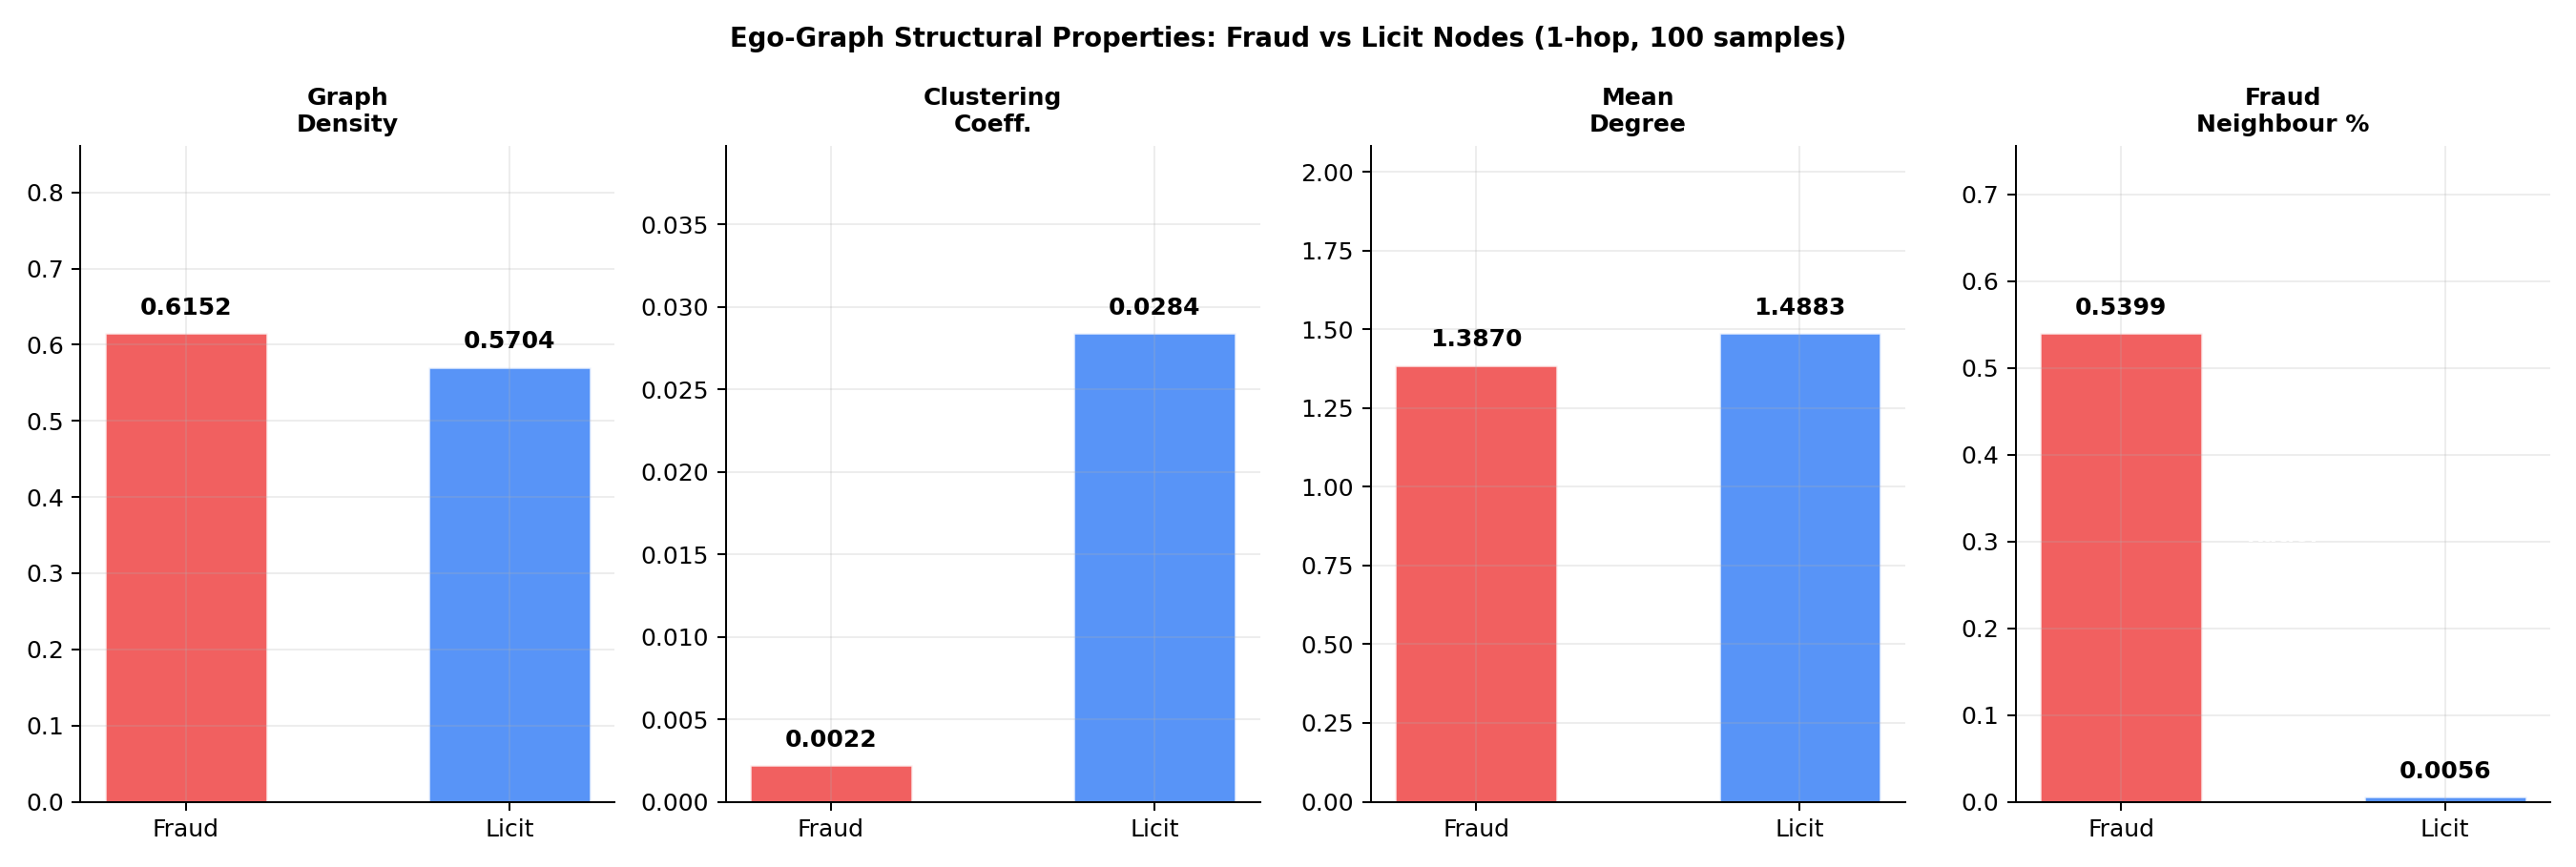
\includegraphics[width=\linewidth]{fig5_community_structure.png}\\[-0.2em]
  \footnotesize\textbf{(a)} Community structure.
\end{minipage}
\hfill
\begin{minipage}[b]{0.32\textwidth}
  \centering
  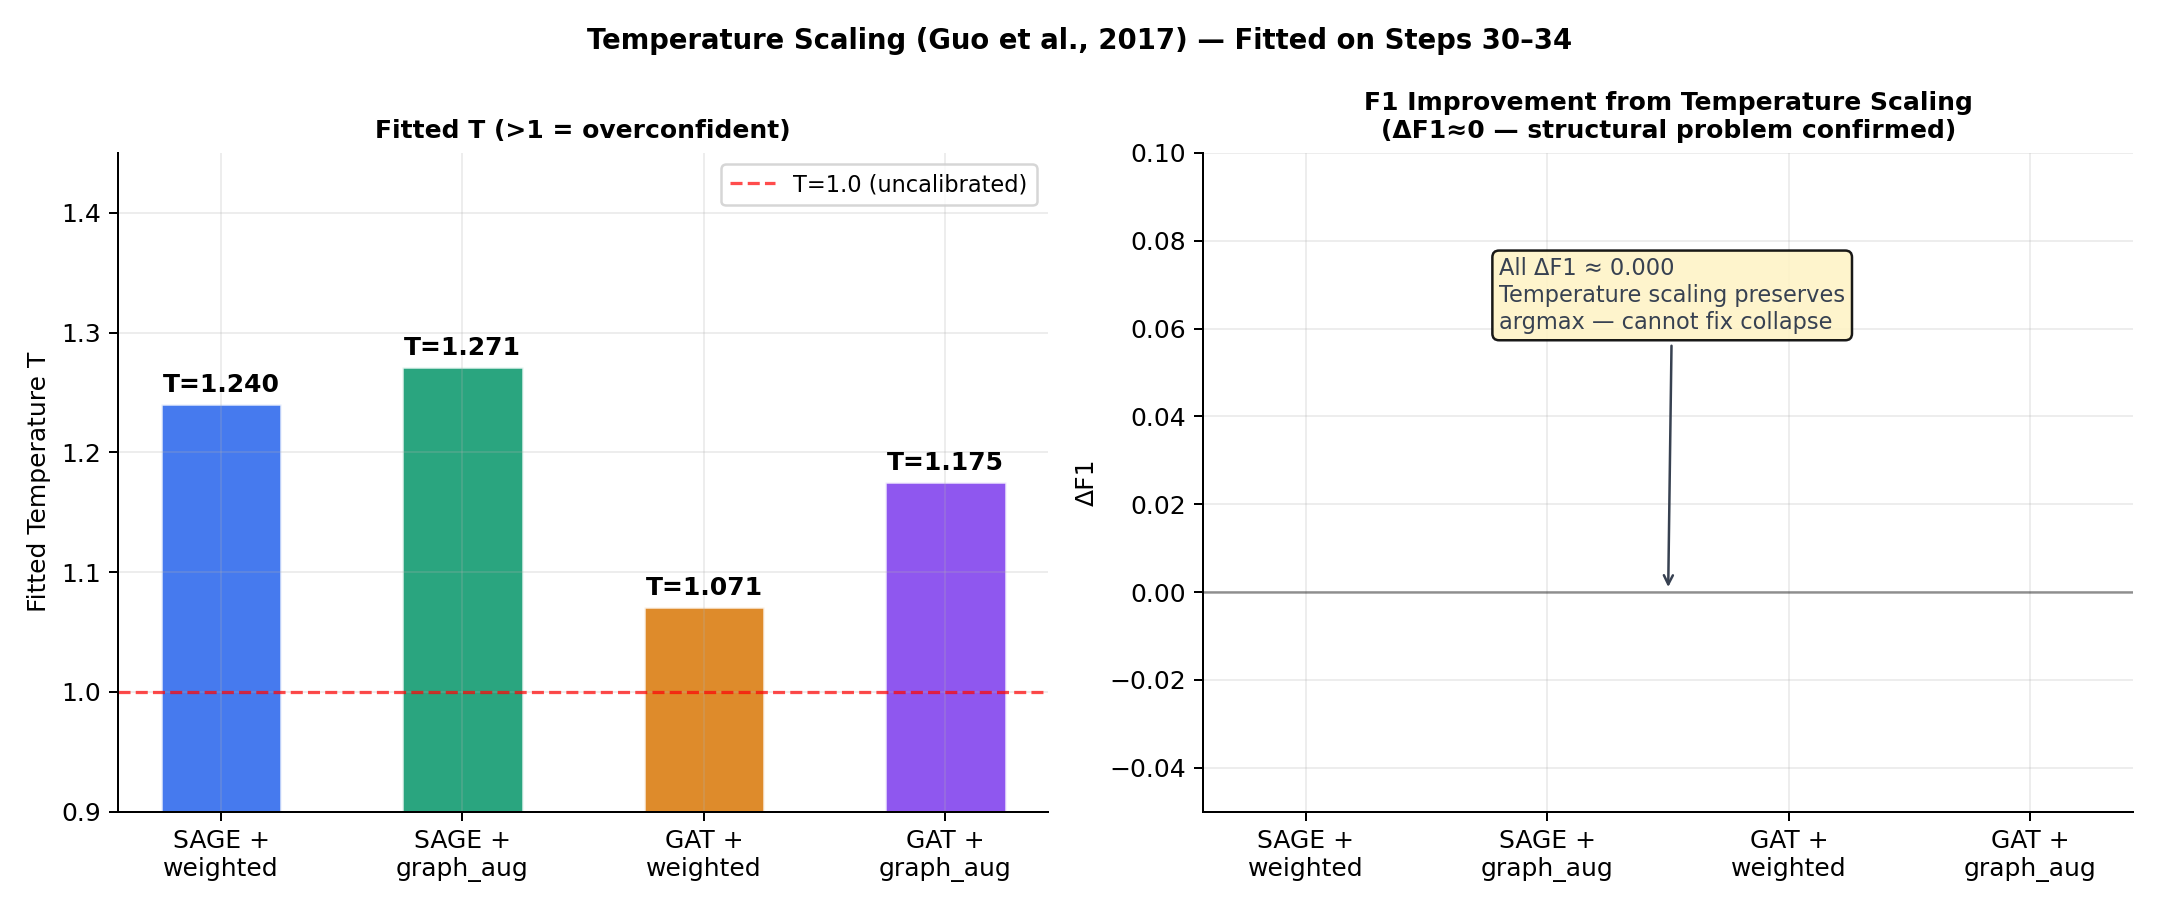
\includegraphics[width=\linewidth]{fig13_temperature_scaling.png}\\[-0.2em]
  \footnotesize\textbf{(b)} Temperature scaling.
\end{minipage}
\hfill
\begin{minipage}[b]{0.32\textwidth}
  \centering
  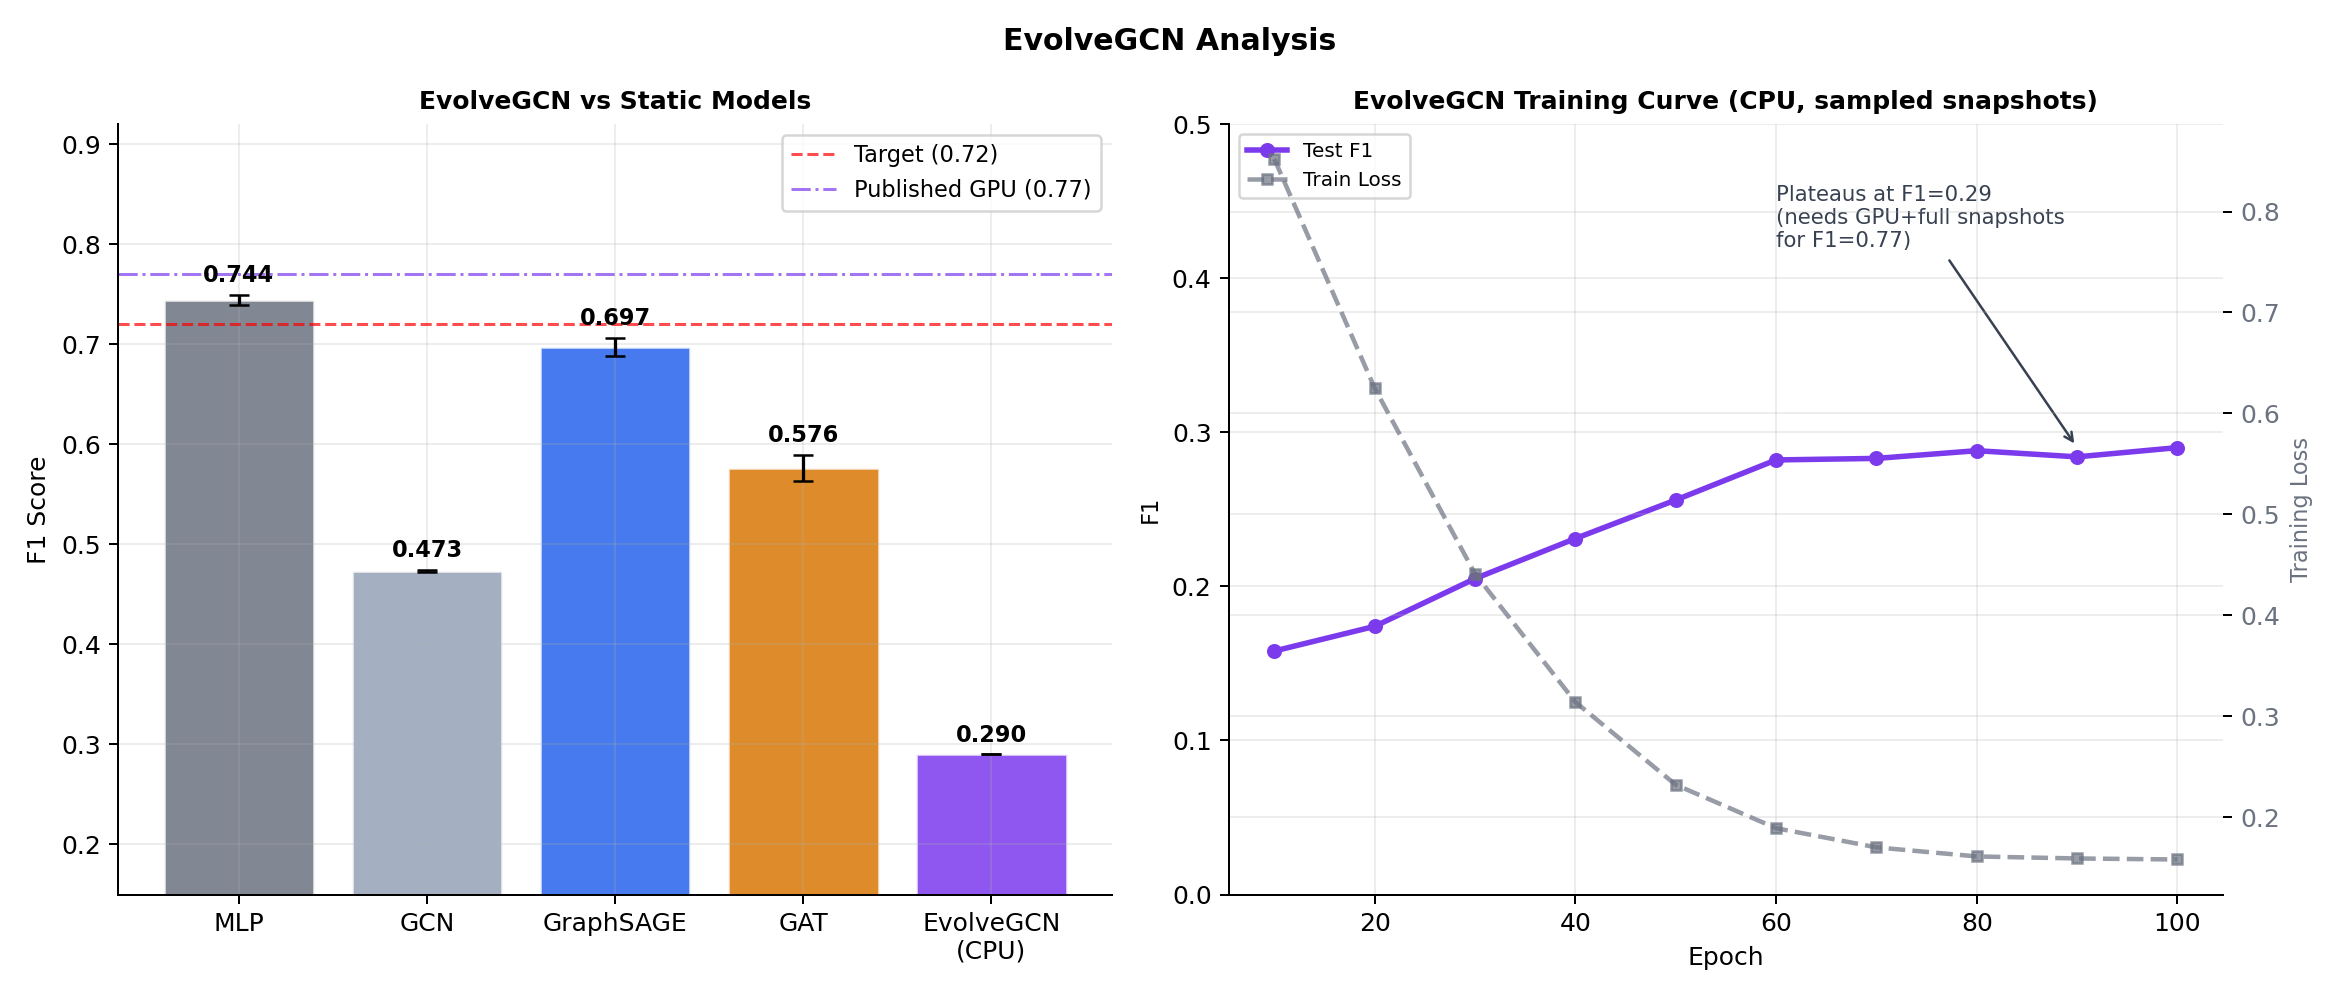
\includegraphics[width=\linewidth]{fig9_evolvegcn.png}\\[-0.2em]
  \footnotesize\textbf{(c)} EvolveGCN hardware ablation.
\end{minipage}
\caption{Three supporting analyses. Fraud communities are real but
  temporally fragile, temperature scaling does not recover performance,
  and temporal GNNs remain highly sensitive to hardware and snapshot
  availability.}
\label{fig:supporting_triptych}
\label{fig:community}
\label{fig:temp}
\label{fig:evolve}
\end{figure*}

\section{Prior Work Comparison}
\label{sec:prior}

Table~\ref{tab:prior} compares our results to published Elliptic work.
All prior studies use GPU hardware and transductive evaluation. Our MLP
(F1\,=\,0.744) matches Alarab et al.\ (F1\,=\,0.740) under stricter
evaluation; our GraphSAGE (F1\,=\,0.697) falls 5.3\,pp below
Lo et al.\ (F1\,=\,0.750), largely due to the transductive-vs-inductive
protocol gap.

\begin{table}[!htbp]
\centering
\caption{Prior Elliptic Work vs.\ This Study}
\label{tab:prior}
\scriptsize
\setlength{\tabcolsep}{3pt}
\begin{tabular}{llrll}
\toprule
\textbf{Work} & \textbf{Model} & \textbf{F1}
  & \textbf{HW} & \textbf{Protocol} \\
\midrule
Weber~\cite{weber2019}    & GCN       & 0.700 & GPU & Transductive \\
Alarab~\cite{alarab2020}  & GCN+feat  & 0.740 & GPU & Transductive \\
Lo~\cite{lo2023}          & SAGE      & 0.750 & GPU & Transductive \\
Pareja~\cite{pareja2020evolvegcn} & EvolveGCN & 0.770 & GPU & Temporal \\
\midrule
\textbf{Ours} & \textbf{MLP} & \textbf{0.744$\pm$.005}
  & CPU & Inductive \\
Ours & SAGE & 0.697$\pm$.009 & CPU & Inductive \\
Ours (ablation) & EvolveGCN & 0.290 & CPU & Sampled \\
\bottomrule
\end{tabular}
\end{table}

\section{Discussion and Conclusion}
\label{sec:conclusion}

\textbf{Three practical implications.} First, periodic retraining is
essential: a 39$\times$ fraud-rate decline cannot be addressed by any
static model or post-hoc calibration. Sliding-window retraining is the
minimum practical requirement. Second, graph structure is a conditional
asset: beneficial in stable periods, harmful under rapid distributional
shift. Adaptive monitoring that switches between structural and
feature-only prediction could capture both benefits. Third, business
cost functions should drive deployment decisions: the highest-F1 model
is not always most cost-effective under asymmetric FN/FP penalties.

\textbf{Limitations.} RandomNodeLoader rather than NeighborLoader
(missing \texttt{torch-sparse} on M4 CPU) may underestimate GNN
performance by 5--10\,pp. Results are from one dataset; generalisation
to other transaction graphs is open. The EvolveGCN result is a hardware
lower bound, not a competitive evaluation.

\textbf{Conclusion.} A plain MLP (F1\,=\,0.744) outperforms all tested
GNNs on the Elliptic Bitcoin Dataset under inductive evaluation. Temporal
distribution shift (fraud rate 11.6\,\% $\to$ 0.3\,\%) causes near-
complete recall failure for all models. Feature importance (82.4\,\%
local feature dominance) explains MLP competitiveness. Temperature
scaling confirms a structural root cause ($\Delta$F1\,=\,0). These
findings motivate periodic retraining and cost-function-driven model
selection for production fraud detection.

\bibliographystyle{IEEEtran}
\bibliography{references}

\end{document}
